%% thesis.tex 2014/04/11
%
% Based on sample files of unknown authorship.
%
% The Current Maintainer of this work is Paul Vojta.

\documentclass[hidelinks]{ucbthesis}
%\usepackage{biblatex}

% To compile this file, run "latex thesis", then "biber thesis"
% (or "bibtex thesis", if the output from latex asks for that instead),
% and then "latex thesis" (without the quotes in each case).

% Double spacing, if you want it.  Do not use for the final copy.
% \def\dsp{\def\baselinestretch{2.0}\large\normalsize}
% \dsp

% If the Grad. Division insists that the first paragraph of a section
% be indented (like the others), then include this line:
% \usepackage{indentfirst}

\setsecnumdepth{subsection} % number sections
\maxtocdepth{subsection}

% Define packages
\usepackage{hyperref, url} 
\usepackage{graphicx,amsfonts,psfrag,layout,subcaption,array,longtable,lscape,booktabs,dcolumn,amsmath,amssymb,amssymb,amsthm,setspace,epigraph,chronology,color,colortbl,wasysym,diagbox,colortbl,authblk,commath,upgreek,natbib}
\usepackage[]{graphicx}\usepackage[]{color}

% Caption keys
\usepackage{mathtools,tikz,caption}
\captionsetup{labelfont=sc,labelsep=period}
\DeclareRobustCommand\sampleline[1]{%
	\tikz\draw[#1] (0,0) (0,\the\dimexpr\fontdimen22\textfont2\relax)
	-- (2em,\the\dimexpr\fontdimen22\textfont2\relax);%
}

\usetikzlibrary{plotmarks}
\usetikzlibrary{automata, positioning}

% Wes Anderson colors

\usepackage{xcolor}

\definecolor{Darjeeling11}{HTML}{FF0000}
\definecolor{Darjeeling15}{HTML}{5BBCD6}

% New footnote characters
\usepackage{footmisc}
\DefineFNsymbols{mySymbols}{{\ensuremath\dagger}{\ensuremath\ddagger}\S\P
	*{**}{\ensuremath{\dagger\dagger}}{\ensuremath{\ddagger\ddagger}}}
\setfnsymbol{mySymbols}

%Rm thanks dagger
\renewcommand\footnotemark{}
%\renewcommand\footnoterule{}

% New tabular environment
\usepackage{tabularx}
\newcolumntype{Y}{>{\raggedleft\arraybackslash}X}% raggedleft column X

% Define appendix 
\renewcommand*\appendixpagename{Appendix}
\renewcommand*\appendixtocname{Appendix}

% Position floats
\renewcommand{\textfraction}{0.05}
\renewcommand{\topfraction}{0.95}
\renewcommand{\bottomfraction}{0.95}
\renewcommand{\floatpagefraction}{0.35}
\setcounter{totalnumber}{5}

% Colors for highlighting tables
\definecolor{Gray}{gray}{0.9}

% Different font in captions
\newcommand{\captionfonts}{\normalsize}

\makeatletter  % Allow the use of @ in command names
\long\def\@makecaption#1#2{%
	\vskip\abovecaptionskip
	\sbox\@tempboxa{{\captionfonts #1: #2}}%
	\ifdim \wd\@tempboxa >\hsize
	{\captionfonts #1: #2\par}
	\else
	\hbox to\hsize{\hfil\box\@tempboxa\hfil}%
	\fi
	\vskip\belowcaptionskip}
%\makeatother   % Cancel the effect of \makeatletter

% Macros
\newcommand{\Adv}{{\mathbf{Adv}}}       
\newcommand{\prp}{{\mathrm{prp}}}                  % How to define new commands 
\newcommand{\calK}{{\cal K}}
\newcommand{\outputs}{{\Rightarrow}}                
\newcommand{\getsr}{{\:\stackrel{{\scriptscriptstyle\hspace{0.2em}\$}}{\leftarrow}\:}}
\newcommand{\andthen}{{\::\;\;}}    %  \: \; for thinspace, medspace, thickspace
\newcommand{\Rand}[1]{{\mathrm{Rand}[{#1}]}}       % A command with one argument
\newcommand{\Perm}[1]{{\mathrm{Perm}[{#1}]}}       
\newcommand{\Randd}[2]{{\mathrm{Rand}[{#1},{#2}]}} % and with two arguments
\newcommand{\E}{\mathrm{E}}
\newcommand{\Var}{\mathrm{Var}}
\newcommand{\Cov}{\mathrm{Cov}}
\DeclareMathOperator*{\plim}{plim}
\newcommand\independent{\protect\mathpalette{\protect\independenT}{\perp}}
\def\independenT#1#2{\mathrel{\rlap{$#1#2$}\mkern2mu{#1#2}}}
\newcommand{\possessivecite}[1]{\citeauthor{#1}'s (\citeyear{#1})} 

\newtheorem{theorem}{Jibberish}

%%%%%%%%%%%%%
%% Chicago 15 ed. author-date
%\usepackage[T1]{fontenc}
%\usepackage[utf8]{inputenc}
%\usepackage[american]{babel}
%\usepackage{csquotes}
%
%\usepackage[authordate,backend=biber,natbib]{biblatex-chicago}
%\addbibresource{references.bib}
%
%% Puts parentheses around year in ref list
%\makeatletter
%\renewbibmacro*{cmsbibyear}{%
%	\printtext[parens]{%
%		\iftoggle{cms@origlabel}%
%		{\usebibmacro{origyear+labelyear}}%
%		{\iftoggle{cms@bothlabelnew}%
%			{\usebibmacro{bothyear+oldstyle}}%
%			{\iftoggle{cms@bothlabelold}%
%				{\usebibmacro{bothyear+oldstyle}}%
%				{\usebibmacro{labelyear+extrayear}}}}}%
%	\ifcsdef{@cms@tempdate}%
%	{\toggletrue{\@cms@tempdate}}%
%	{}}%
%\makeatother

%%%%%%%%%%%%%

\hyphenation{mar-gin-al-ia}
\hyphenation{bra-va-do}

\begin{document}

% Declarations for Front Matter

\title{Essays on the Political Economy of the American Frontier}
\author{Jason V Poulos}
\degreesemester{Spring}
\degreeyear{2019}
\degree{Doctor of Philosophy}
\chair{Professor Sean Gailmard}
\othermembers{Assistant Professor Joshua Blumenstock \\
  Professor Eric Schickler\\
Professor Jasjeet Sekhon}
\numberofmembers{4}
% Previous degrees are no longer to be listed on the title page.
% \prevdegrees{B.A. (University of Northern South Dakota at Hoople) 1978 \\
%   M.S. (Ed's School of Quantum Mechanics and Muffler Repair) 1989}
\field{Political Science}
% Designated Emphasis -- this is optional, and rare
 \emphasis{Computational and Data Science and Engineering}
% This is optional, and rare
% \jointinstitution{University of Western Maryland}
% This is optional
\campus{Berkeley}

% For a masters thesis, replace the above \documentclass line with
% \documentclass[masters]{ucbthesis}
% This affects the title and approval pages, which by default calls this
% document a "dissertation", not a "thesis".

\maketitle
% Delete (or comment out) the \approvalpage line for the final version.
\approvalpage
\copyrightpage

% (This file is included by thesis.tex; you do not latex it by itself.)

\begin{abstract}

% The text of the abstract goes here.  If you need to use a \section
% command you will need to use \section*, \subsection*, etc. so that
% you don't get any numbering.  You probably won't be using any of
% these commands in the abstract anyway.

Your abstract text here. Lorem ipsum dolor sit amet, consectetur adipiscing elit. Nullam
sollicitudin ligula at sapien semper quis consectetur justo consequat. Mauris tristique
vehicula tortor pellentesque auctor. Vivamus metus mauris, convallis sit amet mattis non,
laoreet non lorem. Pellentesque a tempus lacus. Morbi suscipit porttitor tempor. Nulla
facilisi. Morbi nunc erat, imperdiet eget dignissim ac, dictum quis nisl. Aenean viverra
elit sit amet nulla ornare viverra. Vivamus fermentum, nunc in dignissim porta, nibh
tellus viverra lacus, sed malesuada libero purus et velit. Praesent volutpat leo eu risus
rutrum posuere. Etiam cursus ultrices enim. Suspendisse fringilla leo ut ligula dapibus ut
consequat justo vehicula. Ut vulputate, justo in condimentum molestie, orci arcu posuere
urna, vel laoreet augue magna vel tortor. Fusce ut ante lorem, quis dignissim purus. Nam
eget ligula quis sapien scelerisque elementum. Quisque congue tempus ligula, id
consectetur mi congue viverra.


\end{abstract}


\begin{frontmatter}

\begin{dedication}
\null\vfil
\null\hfil
For Mom
\null\hfil
\vfil\null
\end{dedication}

% You can delete the \clearpage lines if you don't want these to start on
% separate pages.

\tableofcontents
%\clearpage
%\listoffigures
%\clearpage
%\listoftables

\begin{acknowledgements}
	
I thank my advisor, Sean Gailmard, for urging me to think more creatively and to pursue outsize research questions. And for reminding me that I'm not my own harshest critic.\\

I acknowledge support of the National Science Foundation Graduate Research Fellowship (DGE 1106400). Part of this work used the computer resources of Stampede2 at the Texas Advanced Computing Center (TACC) under an Extreme Science and Engineering Discovery Environment (XSEDE) startup allocation (TG-SES180010). The Titan Xp GPU used for this part of this research was donated by the NVIDIA Corporation.
\end{acknowledgements}

\end{frontmatter}

%\pagestyle{headings}

%\part{First Part}
\chapter{Introduction}

This dissertation argues that early land reforms had consequential long-run impacts on the development of the American state. The state-building role of land reform, which includes policies to decentralize public land, is frequently discussed in the context of comparative political economy. Several scholars of American Political Development (APD) have studied the implications of land policies designed to open up the western frontier on the developmental trajectory of the U.S. \citep[e.g.,][]{bensel1990,frymer2014rush}; however, this dissertation is the first to quantify how land policies shaped the developmental trajectory of the American political economy.

In the existing APD literature, substantial attention is paid to state-building with respect to the centralization of national power.  For instance, APD scholars trace the expansion of federal bureaucratic capacity through the merit-based federal civil service system installed in the aftermath of the American Civil War \citep{skowronek1982building,bensel1990,carpenter2001}. The American state, however, is organized horizontally and authority is often delegated downward to sub-national units of government. As \citet{novak2008myth} writes, ``trying to gauge the power of the American state or the reach of American public policy by looking simply at the national center or the federal bureaucracy is to miss where much of the action is --- on the local and state levels." How did public land laws shape the development of state governments?

This dissertation also contributes to the comparative politics literature concerned with land reform and state-building  \citep[e.g.,][]{albertus2015autocracy, murtazashvili2016does}. Land reform refers to policies designed to establish or redefine property institutions to increase land tenure, and includes policies such as land redistribution, land titling, and decentralization of public land. 

The essays included in this dissertation explore the consequences to two different mechanisms of public land decentralization in the 19th century U.S.: land lotteries and homestead policies. The latter offered a free land grant to citizens willing to build on an improve a plot of land of predetermined size for a number of years; land lotteries involved the random allocation of the right to file a land grant, without a homesteading requirement. Both were designed to rapidly populate the frontier with mostly white settlers, thereby reducing the costs of defending unsecured territory for a otherwise constrained national and sub-national governments \citep{frymer2014rush}.

\section{Land reform, inequality and state capacity}

Land reform is an important tool of state-building, which is broadly defined as efforts designed to strengthen weak nation-states states through political and economic reforms. It is generally argued in the state-building literature that greater economic power of the ruling class reduces investment in state capacity. State capacity refers not only to the ability to raise revenue, but also the state’s ability to implement policies such as public education through redistributive spending \citep{besley2010state}. The canonical model of \citet{meltzer1981rational} predicts a positive relationship between inequality and redistribution because greater inequality implies the median voter is poorer than the average voter, which in turn increases demand for redistribution in majority-rule elections. 

The canonical model assumes parity in the political influence of voters. However, economic differences in political influence can arise from the comparative advantage of economic elites in solving collective action problems and benefitting from political intervention \citep{acemoglu2008persistence}. Elites have higher education attainment and earnings abilities \citep{bourguignon2000oligarchy}, and their resource advantage and common interests enable them work toward similar policy goals \citep{winters2009}. 

Models that allow for differences in political influence across economic groups yield a nonlinearity in the relationship between inequality and redistribution. In \possessivecite{benabou2000unequal} model, for instance, the pivotal voter is wealthier than the median and has the power to block redistribution as inequality increases. But when inequality is too high, the poor can impose redistribution on elites through `universal' majority voting \citep{perotti1993political,saint1993education}. In \possessivecite{besley2009origins} framework, greater economic power of the ruling class reduces investment in state capacity. 

\citet{galor2009inequality} propose a model where wealthy landowners block education reforms because education favors industrial labor productivity at the expense of the agricultural sector. Their model implies education reforms will not occur where land is abundant and unequally distributed, and thereby delays the transition from an agricultural to an industrial economy. However, land reforms that sufficiently reduce land inequality diminishes the economic incentives of landowners to block education reforms. 
%
%\citet{albertus2015autocracy} theorizes that the successful implementation of land reform requires sufficient administrative capacity, low institutional constraints, and a coalitional split between landowners and the ruling class that provides the ruling class with the incentive to pursue land reform. 

\subsection{``Hollowing out'' tax institutions}
	
Landed elites might choose an inefficient organization of the state in order to create inefficiencies in tax collection \citep{acemoglu2011emergence} or ``hollow-out'' tax institutions in order to constrain the state's ability to tax in the future \citep{suryanarayan2017hollowing}. Inequality in this context can be thought of as a proxy for the amount of \emph{de facto} political influence elites have to block reforms and limit the capacity of the state \citep{acemoglu2008persistence}.

\citet{mares2015non} argue that higher levels of land inequality increases the likelihood of adopting new taxes in order to give the landed elite the ability to design a tax structure that shifts the tax burden from the agricultural sector to the manufacturing sector. The authors show empirically that countries with high levels of land inequality are more likely to adopt the income tax.  Consistent with the findings of \citet{mares2015non}, I show that land inequality is positively related to state capacity, especially at higher levels of inequality. 

This finding is in contrast to several empirical studies that establish a negative relationship between land inequality and state capacity in the context of taxes, revenues, and public school spending at the county-level in 1890 and 1930. These studies are based on analyses over shorter time periods. \citet{ramcharan2010inequality}, for instance, finds an inverse relationship between land inequality and county-level property tax revenues in 1890. The authors find that the negative relationship is especially large in rural counties, where landownership tends to be more concentrated. \citet{vollrath2013inequality} establish a negative relationship between land inequality and local property tax revenues in 1890 in northern rural counties, but not in southern rural counties. 

\section{Culture and migration to the frontier}

It is commonly believed in the political economy literature that state capacity in general is easier to raise in more ethnically or culturally homogeneous societies \citep{besley2010state}. It has also long been viewed in by sociologists \citep{meyer1979public} and more recently, political economists \citep{alesina2013nation,bandiera2018nation}, that the rise of public schooling in the U.S. during the 19th century can be explained as a nation-building policy enacted primarily by state governments, which were the most active level of government in terms of public goods provision from 1790 to the 1840s \citep{wallis2000american}. \citet{bandiera2018nation}, for instance, argues that states adopted compulsory schooling laws as a nation-building tool to instill civic values to the millions of foreign migrants who arrived to the country between 1850 and 1914, during the `Age of Mass Migration.' 

During this time period, the frontier attracted foreign migrants along with workers from eastern U.S. cities, many of whom were the lower end of the skill distribution. \citet{bazzi2017frontier} find evidence that frontier settlers were disproportionately illiterate and foreign-born. The negative selection of westward migrants during this period is consistent with theory of the frontier as a `safety valve' for relieving congested urban labor markets in eastern states \citep{turner1956significance, ferrie1997migration}.

Beside the negative selection in terms of labor market skill, \citet{bazzi2017frontier} argue that the frontier attracted individualists who would be able to thrive in the harsh conditions characterizing the frontier experience; e.g., the social isolation due to low population density on the frontier. The authors find that counties with longer historical frontier experience exhibit lower contemporary property tax rates, and their citizens are more opposed to taxation and redistribution. 

\section{Land monopolization and rent-seeking on the frontier} 

A competing argument emerges from the dissertation that early land reform in the American case increased the economic power of elites by enabling speculators, railroad companies, and other corporations to scoop up huge swaths of valuable land and then act as passive rentiers.  

The U.S. frontier experienced a large-scale transformation of hundreds of millions of public frontier land into private property beginning with the passage of the Land Act of 1820, which permitted the direct sale of public land to private individuals of 80 acres or more for at least \$1.25 an acre, and accelerating after the passage of the homestead acts. About 150 million acres of public land, or about 7\% of the total area of frontier states, had already been sold by the time of the passage of the Homestead Act (HSA) of 1862.\footnote{Source: author's estimates using land patent data described in Section~\ref{state-capacity}.} By the turn of the twentieth century, 250 million acres (11\% of total land area) had been sold, while 100 million acres (4\% of total land area) had been claimed by homestead. In the South, about 50 million acres of public land, or about 31\% of the states' total acreage, had already been sold by before the passage of the Southern Homestead Act of 1866. A substantial rise in the number and total acreage, respectively, of homestead entries in the South and West occurred after the 1889 cash-entry restriction imposed by the U.S. Congress.

The large-scale transfer of public land to railroad companies may have accelerated the increase in frontier land inequality. Land near railroad tracks were often high quality and railroad companies sold excess land to speculators \citep{murtazashvili2013political}. Railroad companies were granted nearly 130 million acres of land between 1862 and 1871 by federal and state governments. About 20\% of the public domain was granted to states or sold or granted to railroads or other corporations, which is comparable to the amount of land granted or sold to homesteaders \citep{shanks2005homestead}.

Speculators and railroad companies worked together to secure state, county, and municipal grants for local railroads. In \possessivecite{gates1939land} study of Indiana counties, for example, speculators fought county governments subsidizing railroads --- despite possibly benefiting from the lines --- and the speculators' land reduced the tax base of the area, so that counties could not sell bonds to finance railroad subsidies. 

\section{``What the railroad will bring us''} 

Frontier states prioritized spending on banking and transportation projects in competition with each other to raise land values and attract more settlers \citep{sylla1998anatomy}. The promise of increasing land values and future tax revenues led frontier states to sharply increase borrowing in the mid-1830s by selling long-term bonds to finance transportation and banking investments. Frontier states in the Northwest (e.g., Illinois, Indiana, and Michigan) borrowed to invest in canals and railroads, while those in the South (e.g, Arkansas, Florida, and Mississippi) borrowed in order to charter state banks. Indiana, for instance, passed the Mammoth Internal Improvement Act in 1836 that added \$10 million in debt spending for transportation projects such as the Wabash and Erie Canal. The state also changed its property tax structure from a flat tax on land to an \emph{ad valorem} tax on all wealth in order to capture the expected increase in land values that would result from the projects \citep{wallis2004sovereign}. The Panic of 1837 decreased land values and put a hole in the state's tax revenue, causing the state to default on its debt and interest obligations.

Because railroads expanded commerce by making it cheaper to trade, railroad access is theoretically expected to increase returns to farm land, and in turn increase the property tax base. \citet{donaldson2016railroads}, for instance, find that average farm values increased substantially as the railroad network expanded from 1870 to 1890, and estimate that the absence of railroads would have decreased farm land values by 60\%. \citet{atack2011impact} attribute two-thirds of the increase in improved farm acreage in Midwestern states to the expansion of railroad access in the decade prior to the Civil War. As evidence that railroad access increases the property tax base through higher land values, \citet{atack2012impact} find school attendance rates increased in counties that gained access to the rail network between 1850 and 1860. 

\section{Counterfactual history}

Inferring causal relationships is a fundamental problem in history and the social sciences. The problem of causal inference is usually framed in terms of counterfactuals: outcomes that would have been observed had the path of history diverged \citep{lewis2013counterfactuals,pearl2009causality,imbens2015causal}. Historians frequently pose counterfactuals in terms of speculating about the `might-have-beens' of history, as it is put by  \citet{elster1978logic}:

\begin{quote}
``In a non-experimental and non-comparative discipline one can hardly discuss the
relative importance of causes without engaging in some kind of thought experiment where one removes successively and separately each of the causes in
question and evaluates what difference the absence of this cause would have
made to the phenomenon in question. Some historians have come to recognize,
therefore, that they have been talking counterfactually all the time without
recognizing it.''
\end{quote}

This dissertation focuses on counterfactual questions in observational studies, where interventions and outcomes have already been recorded. In observational studies, interventions are not randomly assigned and thus there is no ``reasoned basis for inference'' for evaluating counterfactuals, according to Fisherian view of causal inference \citep{fisher1935}. This absence of randomization has not prevented political scientists from reasoning about counterfactuals in comparative case studies \citep{fearon1991counterfactuals, tetlock1996counterfactual,abadie2010synthetic,abadie2015comparative}.% Economic historians have evaluated counterfactual questions such as, ``What would the U.S. economy have been like in 1890 had there been no railroads?'' using a ``social saving" methodology \citep{fogel1964railroads, donaldson2016railroads} or general equilibrium models \citep{williamson2008late}.

\section{Sample selection bias and covariate shift}
The problem of counterfactual analysis in observational studies is inevitably confronted with sample selection bias \citep{heckman1979sample} which arises because the units choose whether they are exposed to treatment, or because the researcher makes nonrandom sample selection decisions. In either case, inferences on observed samples are biased because they differ from what we would infer on random samples from the population. 

The observational study in Chapter \ref{ga-lottery} makes the case that bias due to self-selection is ignorable because the treatment in the study -- winning land in the first two Georgia land lotteries --- was perfectly randomized by the state of Georgia; i.e., it is a true ``natural experiment.'' In Chapters \ref{land-reform} and \ref{rnns-causal}, it is acknowledged that treatment --- exposure to homestead policy or homestead entries authorized by those policies --- is not randomly assigned and units have selected into treatment. Both of these studies approach the problem of causal inference by counterfactual prediction via machine learning methods. The machine learning methods predict counterfactual outcomes of the treated units, which are then compared to the observed outcomes for estimating casual effects. These methods are data-driven, in that they do not require domain knowledge or pre-intervention covariates to generate counterfactual outcomes.  

In machine learning terms, the sample selection bias problem occurs when test set data are drawn from a true distribution and training data are drawn from a biased distribution, where the support of biased distribution is included in that of the true distribution \citep{cortes2008sample}. The sample selection bias problem is a special case of the covariate shift problem, when the distributions of training and test sets differ \citep{bickel2007discriminative}. 

The problem of causal inference by counterfactual prediction assumes that the training set (i.e., control unit observations) and test set (i.e., treated unit observations) are drawn from the same distribution and therefore, requires inference on a different distribution than training set. The approach described in Chapter \ref{rnns-causal} reweights the training loss function by the propensity score \citep{rosenbaum1983central}.\footnote{Note that the propensity score reweighting of the training loss can also be used to correct for the fact that treatment propensity increases over time in staggered treatment adoption settings, such as in Chapter \ref{land-reform}.} This correction technique, along with other regularization approaches, prevent the model from learning an overreliance on certain control units or time periods when generalizing from the factual to counterfactual domains \citep{johansson2016learning}.
	
\section{Overview}

The dissertation is comprised of the following three essays on the political economy of the American frontier. 

\paragraph{State-Building through Public Land Disposal? An Application of Matrix Completion for Counterfactual Prediction}
The essay applies a matrix completion method to predict the counterfactual time-series of frontier state capacity had there been no homestead acts. Causal estimates signify that homestead policies had significant and long-lasting negative impacts on state government expenditure and revenue that lasted a century following their implementation. These results are similar to difference-in-difference (DID) estimates that exploit variation in the timing and intensity of homestead entries aggregated from 1.46 million individual land patent records.

The direction of these estimates align with the view that homestead policies were exploited by land speculators and natural resource companies and that the rents from public land were appropriated by the private sector. I explore land inequality as a possible causal mechanism underlying the relationship between land reform and state capacity, and provide evidence of a positive relationship between land inequality and state government finances and that the slope of correlation increases at higher levels of inequality. I also present DID estimates that reveal per-capita homesteads significantly lowered land inequality in frontier states. The negligible magnitude of the effect suggests that the homesteads did not sufficiently lower land inequality on the frontier, which can explain the negative impacts on state capacity. 

This essay makes a methodological contribution in applying matrix completion for estimating causal impacts of policy interventions on panel data. The method can be easily understood within the framework of modern causal inference, is adaptable to settings with staggered treatment adoption, and outperforms several other regression-based estimators in a battery of placebo tests.

\paragraph{Land Lotteries, Long-term Wealth, and Political Selection} 
This essay asks whether personal wealth can cause individuals to select into office. This question is important and relevant because wealthy individuals might select into office in order to use their power to protect vested interests rather than advance the interests of their constituents. While several studies have studied the effect of officeholding on wealth accumulation, research on the extent to which personal wealth affects the probability of officeholding is much more limited.

The essay takes advantage of the random assignment of land in Georgia at the beginning of the nineteenth century. This random assignment of land generates a meaningful ex-ante exogenous shock to personal wealth, which is expected to reduce the opportunity costs of holding office and may make it more important for the wealthy to hold office. I find no evidence in support of the hypotheses that wealth increases the probability of running for office or holding office and argue that these null results are informative because the estimated effects are not practically different than zero. The absence of a treatment effect suggests that observed cross-sectional correlations between wealth and officeholding are likely due to selection effects. 

\paragraph{RNN-Based Counterfactual Prediction, with an Application to Homestead Policy and Public Schooling}

This essay makes a methodological contribution in proposing a novel alternative to the SCM for estimating the effect of a policy intervention on an outcome over time. The proposed method based on recurrent neural networks (RNNs) is less susceptible to $p$-hacking because it does not require the researcher to choose predictors or pre-intervention covariates to construct the synthetic control. Moreover, RNNs do not assume a functional form, can learn nonconvex combinations of control units, and are specifically structured to exploit temporal dependencies in sequential data.

The RNN-based estimators require sufficient pre-period observations in order to learn an informative representation of the control units, and consequently perform comparatively worse than the SCM on small-dimensional datasets such as those featured in the original synthetic control papers. The RNN-based methods outperform the SCM in high-dimensional data settings when the number of pre-intervention time periods exceeds the number of control units.

In the empirical application, I estimate the causal impacts of the HSA on state government education spending. I find that homestead policy had positive long-run impacts on public education spending, although the impacts are not statistically significant when averaging across the entire post-intervention period. Time-specific causal estimates suggest that the HSA had positive and significant impacts on state government education spending fifty years after the first homestead entry in 1869. The estimated increase in education spending attributable to homestead policy translates to about 3\% of the total school expenditures per-capita in 1929. % Introduction and background to the general topic area.
\chapter{State-Building through Public Land Disposal? An Application of Matrix Completion for Counterfactual Prediction}\label{land-reform}

\begin{quote}  
	\textbf{Summary:} How would the frontier have evolved in the absence of homestead policies? I apply a matrix completion method to predict the counterfactual time-series of frontier state capacity had there been no homesteading. In placebo tests, the matrix completion method outperforms synthetic controls and other regression-based estimators in terms of minimizing prediction error. Causal estimates signify that homestead policies had significant and long-lasting negative impacts on state government expenditure and revenue. These results are similar to difference-in-difference estimates that exploit variation in the timing and intensity of homestead entries aggregated from 1.46 million individual land patent records.
\end{quote}

\section{Introduction}
\noindent
Political scientists are increasingly interested in patterns of state development across time and place. Several scholars \citep[e.g.,][]{bensel1990,murtazashvili2013political,frymer2014rush} theorize a relationship between mid-nineteenth century public land policies and the development of the state, arguing that policies designed to transfer public land to private individuals increased the bureaucratic capacity of the U.S. federal government to administer land. 

Public land policies had long-lasting impacts on state capacity, or the ability of governments to finance and implement policies \citep{besley2010state}. I explore the role of two U.S. public land policies in shaping state capacity: the Homestead Act (HSA) of 1862, which opened for settlement hundreds of millions of acres of western frontier land, and the Southern Homestead Act (SHA) of 1866, which opened over 46 million acres of land for homesteading. I provide evidence that homesteads authorized under these laws had significant long-run impacts on the capacity of frontier state governments. 

The view that the western frontier had long-lasting impacts on the evolution of democratic institutions can be traced to \citet{turner1956significance}. Turner's ``frontier thesis" posited that homestead policies acted as a ``safety valve'' for relieving pressure from congested urban labor markets in eastern states. The view of the frontier as a ``safety valve'' has been explored by \citet{ferrie1997migration}, who finds evidence in a linked census sample of substantial migration to the frontier by unskilled workers and considerable gains in wealth for these migrant workers. Homestead policies not only offered greater economic opportunities to eastern migrants, but also the sparse population on the western frontier meant that state and local governments competed with each other to attract migrants in order to lower local labor costs and to increase land values and tax revenues. Frontier governments offered migrants broad access to cheap land and property rights, unrestricted voting rights, and a more generous provision of schooling and other public goods \citep{engerman2005evolution}.

\citet{garcia2008myth} test the frontier thesis in a global context and conclude that the economic effect of the frontier depends on the quality of political institutions at the time of frontier expansion. Frontier expansion promotes equitable outcomes only when societies are initially democratic. When institutional quality is weak, the existence of frontier land can yield worse developmental outcomes because non-democratic political elites can monopolize frontier lands. Historical scholars have noted that public land policies were often exploited by land speculators, ranchers, miners, and loggers, to accumulate public land and extract natural resources during the early stages of capitalist development \citep{gates1942role,murtazashvili2013political}. According to this view, homesteading laws were \emph{de jure} social polices but \emph{de facto} corporate welfarism. 

The paper makes a methodological contribution in applying an alternative method for estimating causal impacts of policy interventions on time-series cross-section data. Building on a new literature that uses machine learning algorithms such as L1-regularized linear regression \citep{doudchenko2016balancing} or deep neural networks \citep{poulos2017rnn} for counterfactual prediction, I apply a matrix completion method to predict the treated unit time-series in the absence of the intervention. I perform placebo tests and find that the matrix completion method outperforms the synthetic control method and other regression-based estimators in terms of minimizing prediction error. In addition, I show how to evaluate the overall effect of the policy intervention using a randomization inference procedure in which approximately unbiased $p$-values are obtained under minimal assumptions.

The paper proceeds as follows: in Section \ref{history-ch1}, I overview the historical context of homestead policies and its relationship to state capacity and land inequality; Section \ref{estimation} describes the method of matrix completion for counterfactual prediction, benchmarks the method against alternative estimators, and describes the inferential procedure. In Section \ref{state-capacity}, I report the results of placebo tests to verify the consistency of the matrix completion estimator. I then present estimates of the long-run impacts of homestead policies on state capacity. Section~\ref{DID} reports DID estimates of the effect of homesteads on state capacity and land inequality, and Section~\ref{discussion-ch1} concludes. 

\section{Historical background} \label{history-ch1}

The 1862 HSA opened up hundreds of millions of acres of western public land for settlement. The HSA provides that any adult citizen --- including women, immigrants who had applied for citizenship, and freed slaves following the passage of the Fourteenth Amendment---  could apply for a homestead grant of 160 acres of frontier land. Applicants were required to live and make improvements on the land for five years before filing to claim a homestead land grant. 

Under the HSA, the bulk of newly surveyed land on the western frontier was reserved for homesteads, although the law did not end sales of public land. The explicit goal of the HSA was to liberalize the homesteading requirements set by the Preemption Act of 1841, which permitted individuals already inhabiting public land to purchase up to 160 acres at \$1.25 per acre before the land was put up for sale. The implicit goal was to promote rapid settlement on the western frontier and reduce federal government's enforcement costs \citep{allen1991homesteading}. 

In the pre-Reconstruction South, public land was not open to homestead but rather unrestricted cash entry, which permitted the direct sale of public land to private individuals of 80 acres or more for at least \$1.25 an acre. The 1866 SHA restricted cash entry and reserved for homesteading over 46 million acres of public land, or about one-third of the total land area in the five southern public land states (PLS) \citep[pp. 13]{lanza1999agrarianism}. PLS are states created out of the public domain. In the South, these states include Alabama, Arkansas, Florida, Louisiana, and Mississippi. Western PLS include the 25 states that comprise the Midwestern, Southwestern, and Western U.S. (except Hawaii). 

Homestead policies were often exploited by speculators and corporations through fraudulent filings. Speculators and corporations engaged in the practice of paying individuals to stake out homesteads in order to extract resources from the land with no intention of filing for the final patent. In the South, these ``dummy entry-men'' were used by timber and mining companies to extract resources while the cash entry restriction of the SHA was in effect. When the restriction was removed, there was no need for fraudulent filings because the larger companies could buy land in unlimited amounts at a nominal price \citep{gates1940federal, gates1979federal}. The same pattern of fraudulent filings existed in the West, where \citet{murtazashvili2013political} argues that speculators benefited disproportionately from public land policies because the economic balance of power tilted toward the wealthy. \citet{gates1942role} characterizes western speculators who bought land in bulk prior to the 1889 restriction as being influential in state and local governments, resistant to paying taxes, and opposed to government spending. 

\section{Matrix completion for counterfactual prediction} \label{estimation}

An important problem in the social sciences is estimating the effect of a binary intervention on an outcome over time. When interventions take place at an aggregate level (e.g., a state), researchers make causal inferences by comparing the post-intervention (``post-period'') outcomes of affected (``treated'') units against the outcomes of unaffected  (``control'') units. A common approach to the problem is the synthetic control method, which predicts the counterfactual outcomes of treated units by finding a convex combination of control units that match the treated units in term of lagged outcomes. Correlations across units that are assumed to remain constant over time. 

This paper applies the method of matrix completion via nuclear norm minimization (MC-NNM) proposed by \citet{athey2017matrix} to predict counterfactual outcomes. Matrix completion methods \citep[e.g.,][]{mazumder2010spectral} exploit correlations within and across units, but ignore the temporal dimension of the data. These methods typically assume missing values are sampled uniformly at random \citep{yoon2018estimating}; in contrast, the MC-NNM estimator allows for patterns of missing data to have a time-series dependency structure. 

Let $Y$ denote a $\text{N} \times \text{T}$ matrix of outcomes for each unit $i =1, \ldots, \text{N}$ at time $t = 1, \ldots, \text{T}$. $Y$ is incomplete because we observe each element $Y_{it}$ for only the control units and the treated units prior to time of initial treatment exposure, $\text{T}_0$. Let $\mathcal{O}$ denote the set of $(it)$ values that are observed and $\mathcal{M}$ the set of $(it)$ missing values. Let the values of the $\text{N} \times \text{T}$ complete matrix $M$ be $M_{it} =1 $ if $(it) \in \mathcal{M}$ and $M_{it} = 0$ if $(it) \in \mathcal{O}$. Note that the process that generates $M$ is referred to the assignment mechanism in the causal inference literature \citep{imbens2015causal} and the missing data mechanism in missing data analysis \citep{little2014}.

We cannot directly observe counterfactual outcomes and we instead wish to impute missing values in $Y$ for treated units with $M_{it}=1$. In an observational setting, units are part of the assignment mechanism that generates $M$ and patterns of missing data follow one of two specific structures. In the case of simultaneous adoption of treatment, a subset of units are exposed to treatment at time $\text{T}_0$ and every subsequent period. The second structure arises from the staggered adoption setting, where $\text{T}_0$ may vary across treated units. In either case, there are selection biases because the probability of missingness may depend on the unobserved data. The goal is to accurately estimate the effect of a policy intervention despite incomplete data subject to selection bias. 

\subsection{Matrix completion estimator}

Matrix completion methods attempt to impute missing entries in a low-rank matrix by solving a convex optimization problem via NNM, even when relatively few values are observed in $Y$ \citep{candes2009exact,candes2010matrix}. The MC-NNM estimator is 

\begin{equation}
Y_{it} = L_{it}^{*} + \sum_{p=1}^{\text{P}} X_{ip} \upbeta_{p}^{*} + \upgamma_{i}^{*} + \updelta_{t}^{*} + \upepsilon_{it} \label{eq:mc-Y}
\end{equation}

\noindent
where $L^{*}$ a low-rank matrix to be estimated, $X$ is a $\text{N} \times \text{P}$ matrix of normalized, unit-specific covariates, and $\boldsymbol{\upgamma}^{*}$ and $\boldsymbol{\updelta}^{*}$ are vectors of unit and time effects, respectively. The identifying condition is that, conditional on $L^{*}$, the error vector $\boldsymbol{\upepsilon}$ is independent across rows (units) and $\E[\boldsymbol{\upepsilon} | L^{*} + \boldsymbol{\upbeta}^{*} + \boldsymbol{\upgamma}^{*} + \boldsymbol{\updelta}^{*}] = 0$. Estimating $L^{*}$ involves minimizing the sum of squared errors via nuclear norm regularized least squares:

\begin{equation}
\hat{L}, \, \hat{\upbeta} = \min_{L, \,\boldsymbol{\upbeta}} \Bigg[\sum_{(it) \in \mathcal{O}} \frac{1}{|\mathcal{O}|} \bigg(Y_{it} - L_{it} - \sum_{p=1}^{\text{P}} X_{ip} \upbeta_p - \upgamma_{i} - \updelta_{t} \bigg)^2 + \lambda \norm{L}_\star \Bigg], \label{eq:mc-opt}
\end{equation}

\noindent
where $\lambda$ is the regularization term on the nuclear norm $\norm{\cdot}_\star$ --- i.e., sum of singular values --- and its value is selected by cross-validation. The algorithm for (\ref{eq:mc-opt}) iteratively replaces missing values with those recovered from a singular value decomposition (SVD) \citep{mazumder2010spectral}. \citet{amjad2018robust} propose an alternative approach of approximating $L^{*}$ via SVD, and then using linear regression on the ``de-noised'' matrix, rather than relying on matrix norm regularizations.

\citet{athey2017matrix} note two drawbacks of the MC-NNM estimator: first, it penalizes the errors for each value with $M_{it} = 0$ equally without regard to the fact that $\Pr (M_{it}) = 1$ (i.e., the propensity score) increases with $t$. Second, the columns of $\boldsymbol{\upepsilon}$ may be autocorrelated because the estimator does not account for time-series dependencies in the observed data.

\subsection{Simulations} \label{sims}

In this section, I evaluate the accuracy of the MC-NNM estimator on the following three datasets common to the synthetic control literature, with the actual treated unit removed from each dataset: \possessivecite{abadie2003economic} study of the economic impact of terrorism in the Basque Country during the late 1960s ($\text{N}=16$, $\text{T}=43$); \possessivecite{abadie2010synthetic} study of the effects of a large-scale tobacco control program implemented in California in 1988 ($\text{N}=38$, $\text{T}=31$); and \possessivecite{abadie2015comparative} study of the economic impact of the 1990 German reunification on West Germany ($\text{N}=16$, $\text{T}=44$). For each trial run, I randomly select half of the control units to be treated and predict their counterfactual outcomes for periods following a randomly selected $\text{T}_0$. I compare the predicted values to the observed values by calculating the root-mean squared error, $\text{RMSE} = \sum_{it}|L^{*} -\hat{L}|^2 / \sqrt{\text{NT}}$. 

I benchmark the MC-NNM estimator against the following methods:

\begin{description}
		{\setlength\itemindent{1mm}
			\item[(a) DID] Regression of $Y$ on $\boldsymbol{\upgamma}$ and $\boldsymbol{\updelta}$ and a binary treatment variable \citep{athey2017matrix}
			\item[(b) HR-EN] Horizontal regression with elastic net regularization \citep{athey2017matrix} 
			\item[(c) PCA] Regularized iterative principal components analysis \citep{ilin2010practical}
			\item[(d) SC-ADH] Synthetic control approached via exponentiated gradient descent \citep{abadie2010synthetic}
			\item[(e) SVD] Low-rank SVD approximation estimated by expectation maximization \citep{troyanskaya2001missing}
			\item[(f) VT-EN] Vertical regression with elastic net regularization \citep{athey2017matrix}.
		}
\end{description}

Figure \ref{synth-stag} reports the average prediction error of the estimators in a staggered treatment adoption setting, with the estimates jittered horizontally to reduce overlap. Error bars represent 95\% prediction intervals calculated using the standard deviation of the prediction distribution for 20 trial runs. 

Across all estimators, the average RMSE decreases and prediction intervals narrow as $\text{T}_0/\text{T}$ approaches unity because the estimators have more information to generate counterfactual predictions. The MC-NNM estimator generally outperforms all other estimators in terms of average RMSE across different ratios $\text{T}_0/\text{T}$.  The strong performance of the MC-NNM estimator can be attributed to the fact that it is capable of using additional information in the form of pre-intervention (``pre-period'') observations of the treated units, whereas the regression-based estimators rely only on the pre-period observations of control units to predict counterfactuals. Figure \ref{synth-sim} presents a similar pattern of results in a simultaneous adoption setting.

\begin{figure}[htbp]
	\centering
	\begin{subfigure}[t]{0.42\textwidth}
		\centering
		\includegraphics[width=\textwidth]{/media/jason/Dropbox/github/land-reform/paper/plots/basque-stag.png}
		\caption{Basque Country terrorism data, $\text{N}_t = 8$} 
	\end{subfigure}
	~ 
	\begin{subfigure}[t]{0.42\textwidth}
		\centering
		\includegraphics[width=\textwidth]{/media/jason/Dropbox/github/land-reform/paper/plots/california-stag.png}
		\caption{California smoking ban data, $\text{N}_t = 19$}
	\end{subfigure}
	~ 
	\begin{subfigure}[t]{0.42\textwidth}
		\centering
		\includegraphics[width=\textwidth]{/media/jason/Dropbox/github/land-reform/paper/plots/germany-stag.png}
		\caption{West German reunification data, $\text{N}_t = 8$}
	\end{subfigure}
	\caption{Placebo tests under staggered treatment adoption: {\protect\tikz \protect\draw[color={rgb:red,4;green,0;yellow,1}] (0,0) -- plot[mark=o, mark options={scale=1.5}] (0.25,0) -- (0.5,0);}, DID;
		{\protect\tikz \protect\draw[color={rgb:orange,4;yellow,2;pink,3}] (0,0) -- plot[mark=triangle*, mark options={scale=1.5,fill=white}] (0.25,0) -- (0.5,0);}, HR-EN; 
		{\protect\tikz \protect\draw[color={rgb:red,0;green,5;blue,1}] (0,0) -- plot[mark=+, mark options={scale=1.5}] (0.25,0) -- (0.5,0);}, MC-NNM;
		{\protect\tikz \protect\draw[color={rgb:red,0;green,4;blue,2}] (0,0) -- plot[mark=x, mark options={scale=1.5}] (0.25,0) -- (0.5,0);}, PCA;
		{\protect\tikz \protect\draw[color=cyan] (0,0) -- plot[mark=diamond, mark options={scale=1.5}] (0.25,0) -- (0.5,0);}, SC-ADH;
		{\protect\tikz \protect\draw[color={rgb:red,100;pink,100;blue,200}] (0,0) -- plot[mark=triangle, mark options={scale=1.5, rotate=180}] (0.25,0) -- (0.5,0);}, SVD;
		{\protect\tikz \protect\draw[color=magenta] (0,0) -- plot[mark=square, mark options={scale=1.5}] (0.25,0) -- (0.5,0);}, VT-EN.
		\label{synth-stag}}
\end{figure}

\subsection{Hypothesis testing} \label{hyp-test}

Consider a setup with $\text{J}$ control units indexed by $i=1, \ldots, \text{J}$ and $\text{Q}$ treated units indexed by $i = \text{J}+1, \ldots, \text{N}$. The optimization program (\ref{eq:mc-opt}) imputes the missing entries in $Y$:

\[
\hat{Y}_{it} = \hat{L}_{it} \hspace{10mm} \text{for } \text{J}+1 \leq i \leq \text{N} \text{ and } \text{T}_0+1 \leq t \leq \text{T}.
\] The inferred causal effect of the intervention on the treated group is the difference between the observed outcomes of the treated units and the counterfactual outcomes that would have been observed in the absence of the intervention, 

\[
\hat{\alpha}_{it} = Y_{it} - \hat{Y}_{it} \hspace{10mm} \text{for } \text{J}+1 \leq i \leq \text{N} \text{ and } \text{T}_0+1 \leq t \leq \text{T}.
\] Taking the difference-in-means between treated unit observed outcomes and predicted outcomes gives the per-period estimated average causal effect across treated units:

\begin{equation}
\hat{\bar{\alpha}}_{t}  = \frac{1}{\text{Q}} \sum^{\text{N}}_{i=\text{J}+1} \hat{\alpha}_{it} \hspace{10mm}  \text{for } \text{T}_0+1 \leq t \leq \text{T}.  \label{eq:avg-pointwise}
\end{equation}

\citet{chernozhukov2017exact} propose a randomization inference approach for testing the sharp null hypothesis $
\text{H}_0: \boldsymbol{\hat{\bar{\alpha}}} = \boldsymbol{\bar{\alpha}^{o}}$, where $\left\{\bar{\alpha}^{o}_{t}\right\}_{t= \text{T}_0}^\text{T}$ is a trajectory of per-period average effects under the null. The test statistic suggested by the authors is constructed so that we reject higher values:

\begin{equation} \label{tstat}
\text{S}_q (\boldsymbol{\hat{\bar{\alpha}}}) = \left(\frac{1}{\sqrt{\text{T}_\star}} \sum_{t= \text{T}_0 +1}^{\text{T}} |\hat{\bar{\alpha}}_{t}|^q\right)^q,
\end{equation}
%
where $\text{T}_\star = \text{T}- \text{T}_0$ and $q$ is a constant. 

Letting $\boldsymbol{\hat{\bar{\alpha}}_{\pi}}$ denote the vector of per-period average causal effects estimated for each permutation $\pi \in \Pi$, the randomization $p$-value is

\begin{equation}
\hat{p} = 1 - \frac{1}{\Pi} \sum_{\pi \in \Pi} I \left\{\text{S}_q (\boldsymbol{\hat{\bar{\alpha}}_{\pi}}) < \text{S}_q (\boldsymbol{\hat{\bar{\alpha}}}) \right\}, \label{eq:pvalue}
\end{equation}
%
where $I (\cdot)$ denotes the indicator function. 

Following \citet{chernozhukov2017exact}, (\ref{eq:pvalue}) is estimated by permuting $Y$ across the time dimension. The idea for permuting time periods rather than treatment assignment, as proposed by \citet{abadie2010synthetic}, is that if the data are stationary and weakly dependent, which is often the case in an aggregate time-series setting, then the distribution of the error term $\boldsymbol{\epsilon}$ in (\ref{eq:mc-Y}) should be the same in the pre- and post-periods. \citet{chernozhukov2017exact} prove that the $p$-values resulting from their inferential procedure are approximately unbiased under consistent estimation. 

\paragraph{Permuation structures} In the tests described below, three types of permutations are used: i.i.d. random permutations of the time index $t$; i.i.d. block random permutations of $\text{K}=\text{T}/b$ non-overlapping blocks, where $b$ is selected according to the optimal block length for the dependent bootstrap \citep{politis2004automatic}; and moving block permutations that circularly shift $t$ by one period, resulting in $\text{T}-1$ permutations. The latter two permutations are capable of preserving the dependence structure of the data and are thus appropriate for weakly dependent data. 

\section{Impact of homestead policies on state capacity} \label{state-capacity}

In this section, I estimate the causal impacts of homestead policies on state capacity, as measured by state government spending and revenue. I create measures of total expenditure and revenue collected from the records of 48 state governments during the period of 1783 to 1932 \citep{sylla1993sources} and the records of 16 state governments during the period of 1933 to 1937 \citep{sylla1995sourcesa,sylla1995sourcesb}. Comparable measures for 48 states are drawn from U.S. Census special reports for the years 1902, 1913, 1932, 1942, 1962, 1972, and 1982 \citep{haines2010}. The expenditure measure includes state government spending on education, social welfare programs, and transportation. The revenue measure incorporates state government income streams such as tax revenue and non-tax revenues such as land sales.

The data pre-processing steps are as follows. Each measure is inflation-adjusted according to the U.S. Consumer Price Index \citep{williamson2017seven} and scaled by the total free population in the decennial census \citep{haines2010}. Missing values are imputed separately in the pre- and -post-periods by carrying the last observation forward and remaining missing values are imputed by carrying the next observation backward. The raw outcomes data are log-transformed to alleviate exponential effects. Lastly, I remove states with no variance in the pre-period outcomes, resulting in complete $\text{N} \times \text{T}$ matrices of size $33 \times 159$ and $34 \times 158$ for the expenditures and revenues outcomes, respectively. 

In this application, PLS are the treated units and state land states --- i.e., states that were not crafted from the public domain and were therefore not directly affected by homestead policies --- serve as control units. This group includes states of the original 13 colonies, Maine, Tennessee, Texas, Vermont, and West Virginia. The staggered adoption setting is appropriate for the current application because $\text{T}_0$ varies across states that were exposed to homesteads following the passage of the HSA. I aggregate to the state level approximately 1.46 million individual land patent records authorized under the HSA. Land patent records provide information on the initial transfer of land titles from the federal government and are made accessible online by the U.S. General Land Office (\url{https://glorecords.blm.gov}). Using these records, I determine that the earliest homestead entries occurred in 1869 in about half of the western frontier states, about seven years following the enactment of the HSA. In 1872, the first homesteads were filed in southern PLS. The timing and intensity of homestead entries is graphed in Figure \ref{fig:homestead-heatmap}. 

When estimating (\ref{eq:mc-Y}), unit-specific covariates include state-level average farm sizes measured in the 1860 and average farm values measured in the 1850 and 1860 censuses. In theory, we should expect that homesteaders migrate to more productive land and thus excluding these pre-period measures of agricultural productivity may result in overestimating the actual impact of homestead policies. To control for selection bias arising from differences in access to frontier lands, I create a measure of railroad access using digitized railroad maps provided by \citet{atack2013use}, which contain information on the year that each rail line was built. Overlaying the railroad track map over historical county borders, I calculate the total miles of operational track per square mile and aggregate the measure to the state-level.

\subsection{Placebo tests}

Prior to presenting the main results, I assess the validity of the key assumption underlying the approach by discarding post-period observations from the data. Treating $t = \left\{1, \ldots,  \text{T}_0 - \tau\right\}$ as the pre-period, I estimate (\ref{tstat}) and test the zero effect null hypothesis 

\begin{equation} \label{h0-placebo}
\text{H}_0: \text{S}_q (\hat{\bar{\alpha}}_{t}) = 0  \, \hspace{5mm} \,  \text{for} \, \hspace{2mm}  \text{T}_0 - \tau +1 \leq t \leq  \text{T}_0,
\end{equation}
%\frac{1}{\tau +1} \sum_{ \text{T}_0 - \tau +1}^{ \text{T}_0} \hat{\bar{\alpha}}_{t} 
\noindent
where $\tau \in \left\{1, 10, 25\right\}$ and $q \in \left\{1, 2\right\}$. 

Table \ref{placebo-tests} reports randomization $p$-values corresponding to each permutation structure and value of $\tau$ and $q$. i.i.d. block and i.i.d. block $p$-values are calculated using $|\Pi| = 1,000$ permutations. Moving block $p$-values are based on $|\Pi| = \text{T}-1$ permutations. When considering the revenue outcome, placebo tests yield two-sided $p$-values greater than the significance level of $\alpha = 0.05$, regardless of the value of $q$ or permutation structure. These results provide evidence in favor that the model is correctly specified. However, we can only reject the null in the case of $\tau=1$ when considering the expenditure outcome. 

\begin{table}[htbp]
	\captionsetup{font=normalsize}
	\caption{Placebo test $p$-values.\label{placebo-tests}}
	\begin{center}
		\scalebox{.9}{\input{/media/jason/Dropbox/github/land-reform/paper/placebo-tests}}
	\end{center}
\end{table}

Further evidence of the unbiasedness of the estimator is provided in Figure \ref{mc-sim}, which presents the results of placebo tests on control units using both pre- and post-period observations. Similar to the simulations on the synthetic control datasets discussed in Section \ref{sims}, there are no missing entries because the actual treated units are removed prior to the placebo tests. I randomly choose about half of the remaining control units as hypothetical treated units and predict their values for time periods following a randomly selected $\text{T}_0$. The MC-NNM estimator outperforms DID and SVD estimators in terms of minimizing RMSE for each ratio $\text{T}_0/\text{T}$. At $\text{T}_0/\text{T} \geq 0.5$, the estimator generally yields comparable error rates to PCA, synthetic control, and vertical regression estimators. 

\subsection{Main estimates} \label{main-estimates}

In the main analyses, I fit the MC-NNM estimator described in (\ref{eq:mc-Y}) on the entirety of observed entries in $Y$ to recover its missing entries; i.e., the counterfactual outcomes of PLS. The top panel of Figure \ref{mc-estimates-exp-pc} compares the observed time-series of treated units and control units along with the predicted outcomes of treated units. The dashed vertical line represents the initial treatment year of 1869. The observed means of the treated and control units are essentially identical in the post-period. However, we are interested primarily in the difference in the observed and predicted treated unit outcomes, which is the quantity $\hat{\bar{\alpha}}_{t}$, which corresponds to the estimated per-period average causal effect of treatment exposure on the treated units. These per-period causal impacts are plotted in the bottom panels, with 95\% confidence intervals estimated by taking $\hat{\bar{\alpha}}_{t} \pm 1.96$ the standard error of the distribution of 1,000 block bootstrap replicates of $\hat{\bar{\alpha}}_{t}$, with optimal block lengths selected by the procedure described by \citet{politis2004automatic}. 

The per-period impact time-series for both outcomes are essentially zero during the pre-period and within the bounds of the bootstrap confidence intervals, which demonstrates that the model is closely fitting the pre-period observations. Per-period impacts on state government spending peak in 1870, at the same time most PLS were first exposed to homesteads, representing a 0.18 [-0.35, 0.71] log increase in per-capita expenditure. By 1876, after most PLS had been exposed to homesteads, homestead exposure decreases expenditure by 0.51 [-1.67, 0.66] log points, and the trajectory of causal impacts remains negative for the rest of the time-series.

A similar pattern of results emerges when estimating the impacts of homesteads on state government revenue (Figure \ref{mc-estimates-rev-pc}). Per-period impacts on revenue peak in 1873, representing a 0.43 [-0.57, 1.44] log increase in per-capita revenues, at the same time southern PLS are exposed to homesteads. The causal impacts on revenue quickly decrease and remain negative for the remaining time-series; in 1877, exposure to homesteads confer a 0.45 [-1.51, 0.61] log point decrease in per-capita revenue. 

\begin{figure}[htbp]
	\centering
	\includegraphics[width=0.9\textwidth]{/media/jason/Dropbox/github/land-reform/paper/plots/mc-exp-pc.png}
	\caption{MC-NNM estimates of treatment exposure on state government expenditure, 1809 to 1982:
		{\color{Darjeeling15}{\sampleline{}}}, observed treated;
		{\color{Darjeeling11}{\sampleline{dashed}}}, observed control;
		{\color{Darjeeling15}{\sampleline{dotted}}}, counterfactual treated;
		{\color{Darjeeling15}{\sampleline{dash pattern=on .7em off .2em on .05em off .2em}}}, $\hat{\bar{\alpha}}_{t}$.\label{mc-estimates-exp-pc}} 
\end{figure}

The estimated bootstrap confidence intervals are useful for evaluating per-period causal impacts but are not helpful in evaluating the overall effect of homestead policies. Table \ref{mc-estimates} reports the results of testing the null hypothesis:

\begin{equation} \label{h0}
\text{H}_0: \text{S}_q (\hat{\bar{\alpha}}_{t}) = 0  \, \hspace{5mm} \,  \text{for} \, \hspace{2mm}  \text{T}_0 + 1 \leq t \leq \text{T}.
\end{equation}
\noindent

In the table, $\text{S}_q (\boldsymbol{\hat{\bar{\alpha}}})$ corresponds to the test statistic described in (\ref{tstat}) and each value beneath is the randomization $p$-value corresponding to each permutation structure. We can reject the null hypothesis (\ref{h0}) at the 5\% level for both outcomes, both values of $q$, and all three permutation schemes. Note that the relevant test statistic $S (\hat{\bar{\alpha}}_{t})$ measures the trajectory of average causal effects in absolute terms and thus does not provide information on the direction or evolution of the causal effects over time.

\begin{table}[htbp]
	\captionsetup{font=normalsize}
	\caption{Testing the null hypothesis (\ref{h0}).\label{mc-estimates}}
	\begin{center}
		\input{/media/jason/Dropbox/github/land-reform/paper/mc-estimates}
	\end{center}
\end{table}

\section{DID estimation} \label{DID}

The matrix completion approach estimates the impact of a binary exposure to treatment on a continuous outcome. However, in this application a continuous form of treatment is available in the form of homestead entries. Equation (\ref{eq:dd}) estimates a continuous version of the DID estimator described in Section \ref{sims}, where the first difference comes from variation in the date of initial exposure to homesteads, and the second difference comes from variation in the intensity of homestead entries:

\begin{equation} 
Y_{it} =  \gamma_i + \delta_t + \psi \, M_{it} + \phi \, (M_{it} \cdot H_{it}) + X_{it}  + \epsilon_{it}. \label{eq:dd} 
\end{equation}

In this model, $X$ is a matrix of unit- and time-varying covariates included to control for parallel trends in agricultural productivity and access to frontier lands. Entries in the treatment indicator $M$ are set to $M_{it} = 1$ at $t \geq  \text{T}_0$, where $\text{T}_0$ varies across units. The continuous treatment exposure variable $H_{it}$ measures the per-capita statewide sum of homestead entries in state $i$ and year $t$. The coefficient corresponding to the interaction term, $\hat{\phi}$, is the estimated average causal effect of exposure to homesteads. I use unit-stratified bootstrapped samples to construct nonparametric standard errors for $\hat{\phi}$. The model assumes i.i.d. errors, which understates the standard errors for $\hat{\updelta}$ when the regression errors are serially correlated, or $\mathrm{Corr} (\epsilon_{it}, \epsilon_{i,t-1}) \neq 0$, which can arise when the time-series lengths are not sufficiently long to reliably estimate the data generating process. \citet{bertrand2004much} show that the stratified bootstrap can be used to compute consistent standard errors when the number of units is sufficiently large. 

Similar to the case of binary treatment, the continuous DID estimator is adapted to a setting of staggered adoption because the initial date of exposure to homesteads varies across PLS. It should be emphasized that estimating (\ref{eq:dd}) in a staggered adoption setting relies on several strong assumptions regarding both the assignment mechanism --- in this application, the distribution of $\text{T}_0$ --- and the counterfactual outcomes of the treated units. The framework of \citet{athey2018design}, for instance, assumes the distribution of $\text{T}_0$ is completely random conditional on the covariates. In the current application, this assumption ignores the possibility that initial exposure to homesteads might be determined by unobserved factors. The framework also that the counterfactual outcomes at time $t$ does not depend on the future date of treatment exposure if $t <  \text{T}_0$ or the history of treatment exposure if $t >  \text{T}_0$. Violations of these assumptions would arise if the homestead policies is anticipated prior to $\text{T}_0$ or if the size of frontier state government is determined by whether the state was exposed early or late to homesteads. 

\subsection{DID estimates on state capacity}

I estimate (\ref{eq:dd}) on balanced state-year panel datasets of state government finances from the years 1783 to 1982. The covariate matrix $X_{it}$ includes measures of railroad access, farm sizes, and farm values. Missing values in $X_{it}$ are imputed separately in the time periods before and after 1868, carrying the last observation forward and impute remaining missing values by carrying the next observation backward.

Table \ref{dd-estimates} reports the DID treatment effect estimates and corresponding 95\% confidence intervals constructed using 1,000 state-stratified bootstrap samples. The estimates indicate that a 10\% increase in log per-capita homesteads is expected to significantly decrease log per-capita stage government finances by about 0.1\%. The point estimates are considerably smaller in magnitude -- albeit in the the same direction-- as the per-period MC-NNM estimates presented in Section \ref{main-estimates}. The bootstrap confidence intervals around the DID estimates are considerably more narrow than those for the MC-NNM per-period impacts displayed in Figure \ref{mc-estimates} and are potentially overoptimistic due to serial correlation in the DID regression errors.

\begin{table}[htbp]
	\begin{center}
		\caption{DID estimates: Impact of homestead entries on outcomes. \label{dd-estimates}}
		\resizebox{.9\width}{!}{\input{/media/jason/Dropbox/github/land-reform/paper/dd-estimates}}
	\end{center}
\end{table}

\subsection{Land inequality as a causal mechanism}  \label{mechanisms}

Through which channels do homesteads affect state capacity? The political economy literature is largely in agreement that inequality and state capacity are inversely related. In \possessivecite{besley2009origins} framework, for example, greater economic power of the ruling class reduces investment in state capacity. Similarly, \citet{galor2009inequality} propose a model where wealthy landowners block education reforms because education favors industrial labor productivity and decreases the value in farm rents. Inequality in this context can be thought of as a proxy for the amount of \emph{de facto} political influence elites have to block reforms and limit the capacity of the state \citep{acemoglu2008persistence}. 

To test whether homesteads affected future land inequality in frontier counties, I calculate a commonly-used measure of land inequality based on the Gini coefficient of census farm sizes. Gini-based land inequality measures are commonly used as proxy for the \emph{de facto} bargaining power of landed elites \citep[e.g.,][]{boix2003democracy,ziblatt2008does,ansell2015}. Note that the Gini coefficient will underestimate land inequality in counties with high shares of propertyless farmers because tenant farms are included in the farm size data, which is problematic because farms can be operated by different tenants but owned by the same landlord. I correct for this problem by adjusting the farm Gini coefficient by the ratio of farms to adult males, as recommended by \citet{vollrath2013inequality}.

In Figure \ref{fig:ineq-capacity}, a bivariate regression model yields a positive relationship between land inequality and state government finances during the period of 1860 to 1950, especially at higher levels of inequality. This relationship points to inequality as a potential causal mechanism underlying the relationship between homesteads and state capacity. The inverse relationship agrees with the findings of \citet{ramcharan2010inequality} and \citet{vollrath2013inequality} in the context of taxes, revenues, and public school spending at the county-level in 1890 and 1930.

Table \ref{dd-estimates} presents DID estimates of the impact of log per-capita homesteads on land inequality at the state-level during the period of 1870 to 1950. Since land inequality is measured every decennial, I aggregate homesteads to the next decennial year; e.g., the number of homesteads measured in 1880 is the total for the years 1871 to 1880. Average farm values are included in the regression as a proxy for agricultural productivity, which might be associated with farm sizes approaching ideal scale and therefore land inequality. I estimate that homesteads significantly decreased land inequality in frontier states: a 1\% increase in log per-capita homesteads is expected to lower  land inequality by $4.81\,\cdot\,10^{-6}$ points. 

\section{Conclusion} \label{discussion-ch1} 

The findings of this paper signify that mid-nineteenth century homestead policies had long-lasting impacts that can potentially explain contemporary differences in state government capacity. MC-NNM and DID estimates imply that homestead policies --- or the homestead entries authorized by those policies --- had significant and negative impacts on state government expenditure and revenue that lasted a century following its implementation. The direction of these estimates contradicts the view that frontier state governments sought to increase public investments in order to attract eastern migrants following the passage of the HSA, and that homesteads would increase state and local tax bases. Instead, the results conform with the view that homestead policies were exploited by land speculators and natural resource companies and that the rents from public land were appropriated by the private sector. 

I explore land inequality as a possible causal mechanism underlying the relationship between land reform and state capacity. First, I provide evidence of a positive relationship between land inequality and state government finances and that the slope of correlation increases at higher levels of inequality. A nonlinearity in the relationship between inequality and state capacity can arise in theoretical models that incorporate economic differences in political influence: greater income inequality reduces investments in fiscal capacity when elites have a monopoly on political power, however when inequality gets too high, the poor can impose redistribution through majority voting. Second, I present DID estimates that reveal per-capita homesteads significantly lowered land inequality in frontier states; although, the magnitude of the effect is negligible. 

This paper makes a methodological contribution in applying matrix completion --- a machine learning method commonly used for user recommendation tasks --- for estimating causal impacts of policy interventions on time-series cross-sectional data. The promise of the method is three-fold. First, the method can be easily understood within the frameworks of modern causal inference and missing data imputation: we cannot directly observe the counterfactual outcomes of treated units and wish to impute these values on the basis of the observed values. Second, the method allows for patterns of missing data to have a time-series dependency structure and is thus adaptable to settings with staggered treatment adoption. Third, the method outperforms several other regression-based estimators in a battery of placebo tests. The performance advantage can be attributed to the fact that it is capable of using additional information in the form of pre-period observations of the treated units, whereas other estimators rely only on the pre-period observations of control units to predict counterfactuals. 

Further research is needed to determine the conditions under which consistency holds. Estimator consistency is required to obtain approximately unbiased $p$-values under the randomization inference procedure.  % land-reform
\chapter{Using Land Lotteries for Natural Experiments on Wealth and Power} \label{land-lotteries}

The hypothesis that personal wealth influences political power has a long tradition in political theory, but has rarely been systematically studied. \citet{ferguson1767}, for instance, theorizes that unequal divisions of property produce inequalities in political power. \citet{madison1787} similarly argues that representative bodies reflect the sentiments that arise from the unequal distributions of property.\footnote{Madison does not fear the aristocracy; rather, he is more concerned about the possibility of an ``overbearing majority'' of propertyless men that would restrict property rights. For this reason, Madison argued in favor of property qualifications for voters during the Constitutional Convention, concluding, ``the freeholders of the Country would be the safest depositories of Republican liberty.''} \citet{beard1913} argues the framers of the U.S. Constitution designed the document to protect commercial property interests from the reach of popular majorities.\footnote{The specific property interests Beard refers to are ``money, public securities, manufactures, and trade and shipping,'' which were disadvantaged by the Articles of Confederation and instead favored small farmers and debtors. Beard argues the Framers were ``personally interested in, and derived economic advantages from'' the Constitution.} 

It is unclear whether wealth causes elites to seek office and vote in favor of their vested interests, or whether officeholding and the ideology of self-interest are simply correlated with unobserved personal characteristics related to the accumulation of personal wealth. For this reason, observational studies on the relationship between personal wealth or economic class and officeholding or ideology suffer from endogeneity bias. \citet{carnes2012}, for example, finds members of the U.S. House of Representatives with white-collar backgrounds vote more conservatively on economic policy than members with blue-collar backgrounds. \citet{doherty2006} estimates the effect of randomly-induced wealth on economic policy beliefs on Massachusetts lottery winners, finding lottery wealth increases opposition to estate taxes and government redistribution. \citet{rossi2014} exploits the random allocation of land in $16^{th}$ century Argentina to identify the effect of wealth on dynastic officeholding, showing that families receiving more valuable land closer to the city of Buenos Aires have a higher probability of ex-post officeholding. 

These observational studies suffer from sample selection bias due to non-random assignment of experimental groups. Chapter \ref{ga-lottery} explores the relationship between wealth and officeholding using a natural experiment in public land decentralization where land wealth was actually randomly allocated to lottery participants. The random allocation of land wealth allows us to obtain unbiased estimates of the effect of wealth on officeholding. Section \ref{land-lotteries-background} overviews the historical context of the first two Georgia land lotteries, which provide the data for the natural experiment in Chapter \ref{ga-lottery}.% It also overviews the historical background of the only other large-scale land lottery outside of Georgia, occurring in Oklahoma in 1901. Future research could replicate the natural experiment of Chapter \ref{ga-lottery} in the context of the Oklahoma lottery. 

\section{Historical Background of Land Lotteries} \label{land-lotteries-background}

In 1805 and 1807, the state of Georgia conducted the first two public land lotteries in U.S. history, only to be replicated in six subsequent Georgia land lotteries and Oklahoma's 1901 lottery. Approximately two million acres were redistributed in the Oklahoma lottery, compared to more than one million acres in the 1805 lottery, 2.2 million acres in the 1807 lottery, and more than 27 acres in all eight Georgia lotteries \citep{graham2004}. 

\subsection{1805 Georgia Land Lottery}

In 1802, the Creek Nation signed a treaty at Fort Wilkinson ceding territory south of the Oconee and Altamaha rivers. The first mechanism used for decentralizing state lands was the ``headright system'' in which heads of household were entitled to 200 acres of land and additionally 50 acres for each family member or slave (capped at 1,000 acres). The headright system favored the wealthy and well-connected, who could receive more land by obtaining the approval of the Assembly and the Governor, who at the time was appointed by the legislature \citep{meyers2012}. 

The end of the headright system and the birth of the public land lottery followed from two well known scandals. In what is referred to as the Pine Barrens scandal, three different Georgia governors signed off on grants of millions of acres of land --- more than actually existed --- to a few land speculators. The Pine Barrens scandal was followed by the Yazoo Act of 1795, in which the legislature allocated up to 50 million acres of ceded land to four speculation companies for a half-million dollars in return for bribes. Following a public anti-corruption campaign, voters installed a mostly new government in the election of 1796, which quickly nullified the Yazoo Act and grants made under the Act \citep{meyers2012}. 

Georgia's new Assembly responded with a novel system of land redistribution: a public land lottery. The Act of 11 May 1803 outlined the rules and procedures of the 1805 lottery, which served as a model for subsequent Georgia land lotteries. The lottery prevented the accumulation of land by speculators and was inherently less corruptible than the headright system. \citet{chappell1874} remarks, 

\begin{quotation}
	... [E]very temptation and means for the practice of fraud and corruption was taken away. For who was going to bribe the members of the Legislature or other public functionaries, high or low, when it was rendered utterly impossible by the very system adopted, for the corruptor to make or secure anything by means of the bribery?
\end{quotation}

The Act created three new counties using land from the former Creek territories: the territory lying south of the Oconee river was split into two counties, the northern part called Baldwin and the southern part called Wilkinson, with each county divided into five districts; Wayne county, positioned south of the Altamaha river, was divided into three districts \citep{clayton1812}.\footnote{Figure \ref{map} shows the ceded lands that were at stake in the 1805 and 1807 lotteries.}

\begin{figure}[htbp] 
	\centering
	\includegraphics[width=0.8\textwidth]{/media/jason/Dropbox/ga-lottery-local/paper-drafts/paper-sixth/county-map.png} 
	\caption{Map of Georgia with 1807 county boundaries \citep{long1995atlas}. The shaded counties are original counties created by the Acts of 11 May 1803 and 9 June 1806.\label{map}}
\end{figure}

For each district, one surveyor was appointed by the legislature to map the area into square lots and to return the results to the Surveyor General. The Act outlines the process of distributing the surveyed lots in the lottery:

\begin{quotation}
	After the surveying is completed, and the returns made to the Surveyor General, his Excellency the Governor shall cause tickets to be made out whereby all the numbers of the surveys in the different districts shall be represented, which tickets shall be put into a box to constitute prizes, with others to be denominated blanks, of which blanks the number or amount shall be determined, by subtracting the number of prizes from the whole number of draws.
\end{quotation} 

Registration for eligible citizens took place in the eleven months following passage of the law. Eligibility was extended to free white men 21 years and older and orphaned children, each receiving one draw. Married white men with children and widows with children received two draws. Citizens were given at least 10 days notice, by public advertisement, to attend their respective county courthouse in order to register. County justices were responsible for compiling a list of names and number of eligible draws for each registered participant.

The lottery was established under the direction of five managers appointed by the legislature.\footnote{The five managers were Jared Irwin (President), William Barnett, George R. Clayton, Edwin Mounger, and George Watkins. Irwin was a political reformer who, during his first term as Governor of Georgia (1796-1798), signed the bill that nullified the Yazoo Act. Barnett was a state senator from Elbert county. Mounger served as State Treasurer at the time of the lottery (1799-1806). Clayton served as State Treasurer after Mounger (1806-1825). Watkins was a local politician who authored the first \textit{Digest of the Laws of the State of Georgia} with his brother Robert in 1800.} The managers apportioned the blank and prize tickets, which were placed in a wooden ``lottery wheel'' \citep{cadle1991}. The lottery room was arranged with the managers seated at a long table with a volume of four books containing the names of all participants. The managers announced the names and number of registered draws for each participant in alphabetical orde and drew the tickets without replacement as each participant name was announced. For over five weeks, approximately 1,250 tickets were drawn each day (except Sunday) in this manner \citep{graham2004}.

Participants who won a prize, or ``fortunate drawers,'' had 12 months following the drawing to claim their prize. Fortunate drawers were required to pay four dollars per 100 acres in order to obtain the land grant. In some cases, fortunate drawers sold their grants to land speculators, who in turn sold the land to out-of-state settlers \citep{davis1981}. Land speculators often sought out fortunate drawers who drew particularly valuable lots \citep{cadle1991}. The grant records indicate, for instance, 52 grants were obtained jointly by speculators John Forsyth and Lewis Alexander Dugas.\footnote{Forsyth was a Georgia lawyer who launched an illustrious political career in 1808 when he was elected attorney general of Georgia; Forsyth would later serve as the 33rd Governor of Georgia and the 13th U.S. Secretary of State. Dugas was a Georgia businessman. Land speculator Robert Flournoy of Putnam County purchased 36 grants. Flournoy served two consecutive terms as a state senator from Montgomery county starting in 1814.}

\subsection{1807 Georgia Land Lottery}

The Act of 9 June 1806 extended the boundary between Baldwin and Wilkinson counties 45 degrees west to the Ocmulgee River, adding the area north of the line to Baldwin and the area south of the line to Wilkinson \citep{clayton1812}. The surveying process, which was identical to the 1805 lottery, created 38 districts --- 15 to Baldwin and 23 to Wilkinson --- with each square lot of 202.5 acres included in the public lottery. The process of registering participants was similar to the previous lottery, with participants paying 12.5 cents per draw. The eligibility rules were also similar, except that orphan families with both parents deceased received two draws, widows had one draw, free white unmarried females over the age of 21 had one draw, and 1805 fortunate drawers were excluded from participation. 

Unlike the 1805 lottery, there were two lottery wheels used in the 1807 drawing: one containing the names of participants, and the other containing lot numbers. Blank tickets in number equal to difference between the number of registered draws and prize lots were added to the lottery wheel. Tickets from each wheel were drawn simultaneously to form a combined ticket. If the combined ticket included a prize, the winning participant's information was recorded in a grant book. The grant process in the 1807 lottery was similar to that of the 1805 lottery \citep{graham2011}. 
%
%\subsection{1901 Oklahoma Land Lottery} \label{ok-lottery}
%
%At the turn of the 20th Century, the central and western parts of Oklahoma were opened to settlement by non-native Americans. Most of the unassigned lands in central Oklahoma, ceded to the U.S. by the Creek and Seminole Indians following the Civil War, were opened by land run beginning in 1889. In contrast, unassigned land formerly occupied by the Kiowa, Comanche, Apache, and Wichita tribes were opened for settlement by lottery in the summer of 1901 and split into two districts: El Reno and Lawton. 
%
%About 170,000 people registered for the drawing for the chance to win one of 13,000 lots of 160 acres in size.  Registration was open to heads of household 21 years old or older who did not already own more than 160 acres of land. Land officials randomly drew 6,500 envelopes containing participants' information from each of two large hoppers --- one for participants who wanted to claim land in Lawton and the other for those who wanted land in El Reno --- and envelopes were numbered as they were drawn \citep{anderson1997}. Results of the drawing were mailed to participants and posted in the newspapers. Lottery winners had the opportunity to ``stake [a] claim in turn" according to the number on the envelope during the span of 60 days \citep{watson1988}.
%
%Lottery participants were drawn in rank order: the person who drew number one was given first choice, the person who drew number two was given second choice, etc. The draw order was therefore an approximate rank ordering of the amount of lottery wealth, in terms of the option value of the land. \citet{bohanon1998costs} provide a lower-bound estimate of \$496 for the value of a 160-acre lot, which is roughly equal to the average farm income at the time of the 1900 Census. Contemporaneous accounts estimate that the most valuable lots adjacent to the city of Lawton were worth between \$20,000 to \$40,000.\footnote{``Our Uncle Samuel's Lottery and Land Drawing in Oklahoma." \emph{Fort Morgan Times}, Volume XVII, Number 51, August 3, 1901. Available at \url{https://www.coloradohistoricnewspapers.org}.}  % transistion into ga-lottery
\chapter[Land Lotteries, Long-term Wealth, and Political Selection]{Land Lotteries, Long-term Wealth, and Political Selection\footnote{This paper is previously published \citep{poulos2019land}.}}\label{ga-lottery}

\begin{quote}  
	\textbf{Summary:} Does personal wealth cause individuals to select into public office? This study exploits the 1805 and 1807 Georgia land lotteries to investigate the hypothesis that wealth increases political power. Most eligible males participated in the lotteries and more than one-in-ten participants won a land prize worth over half of median property wealth. I find no evidence that lottery wealth increases the likelihood of officeholding or running for office, and argue that those null findings are informative because the estimates are not practically different from zero. The absence of a treatment effect implies that commonly observed cross-sectional correlations between personal wealth and officeholding are likely explained by selection effects.
\end{quote}

\clearpage

\section{Introduction}

\noindent
A problem in representative democracies is that elected officials might use their power to defend vested interests rather than advance the interests of their constituents. Personal wealth is expected to reduce the opportunity costs of holding public office and also may make it more important for wealthy citizens to seek elective or appointive positions. While several studies have examined the effect of officeholding on wealth accumulation  \citep[e.g.,][]{eggers2009,querubin2013,truex2013}, research on the extent to which wealth affects officeholding is more limited. 

Natural experiments that exploit exogenous variation in personal wealth can be used to identify wealth's causal effects on officeholding. State-run lotteries that randomly distribute land titles to individuals satisfy that objective because winning a land title represents an exogenous shock to personal wealth. \citet{rossi2014}, for instance, exploits the random allocation of land in $16^{th}$ century Argentina to identify the causal relationship between wealth and subsequent political power. Wealth is proxied by the distance of randomly allocated land from the City of Buenos Aires, where land closer to the city is more valuable and political power is represented as a binary variable indicating whether heads of household or their relatives held a position in city government. Rossi finds that an increase of one standard deviation in the distance of the land to the city reduces the likelihood of political power by about 12\%.\footnote{The linear model used to obtain the estimate assumes that distance of the land to the city is uncorrelated with unobserved individual-level predictors of political labor supply, such as the opportunity costs associated with holding office.}

The present study uses the first two Georgia land lotteries as natural experiments to investigate the hypothesis that personal wealth increases subsequent political power. The 1805 lottery was the first public land lottery in US history, only to be replicated in 1807 and six later Georgia lotteries.\footnote{The six later Georgia lotteries were held in 1820, 1821, 1827, 1832, 1832 (``Gold Lottery''), and 1833 (``Fractions Lottery'').} The state distributed more than one million acres of land in the 1805 lottery, two million acres in the 1807 lottery, and 23 million acres in all eight lotteries \citep{cadle1991}. A sizable majority of eligible adult white males participated in the lotteries, and about one-in-ten won land prizes with an estimated mean value of least \$800, which represents more than half of median property wealth at the time of the lotteries. Since land prizes could readily be sold in a secondary market for public land, the random assignment of land generates an ex-ante exogenous shock to personal wealth. However, I find no evidence in support of the hypotheses that wealth increases the likelihood of officeholding or political candidacy. I argue that those null results are still informative because the estimates are not practically different from zero. 

Did winning the lottery not affect officeholding or candidacy because the magnitude of the windfall --- while large relative to average wealth --- was not sufficient to move the median participant into the slaveholding elite that formed the largest political class in the antebellum South? To determine  whether treatment translates into long-run wealth for lottery winners, I link the participant records to the full-count 1820 Census, which is the earliest census to include a measure of individual wealth: the number of slaves owned. I provide evidence from quantile regression estimates that winning a prize in the 1805 lottery conferred on lottery winners near the median of the wealth distribution a \$171 increase in wealth, with a 95\% confidence interval of [\$18, \$323]. The upper bound of the estimate is enough wealth to satisfy the freehold qualification for running for representative to Georgia's legislature. The estimate is similar in size to \possessivecite{bleakley2013up} estimate that winning a prize in the 1832 Georgia lottery significantly increases 1850 total census wealth (i.e., combined slave and real-estate wealth) by \$200.\footnote{The authors use a sample of 1832 lottery participants linked to the full-count 1850 Census to investigate the effects of lottery prize values on the long-run wealth distribution of lottery winners. Using the same linked sample, \citet{bleakley2016} finds no evidence of a treatment effect on the wealth, literacy, or occupational standing of lottery winners or their descendants.} 

This paper proceeds as follows: Section \ref{theory} provides a theoretical discussion of the channels through which wealth may or may not impact political power; Section \ref{history-ch2} provides some historical background, including details on the development and implementation of the 1805 and 1807 lotteries. Section \ref{data} describes the data and record-linkage procedure, and provides summary statistics on the wealth of officeholders. Section \ref{results} specifies the treatment effect estimator, tests the assumption of random treatment assignment, and provides treatment effect estimates. Section \ref{discussion-ch2} discusses concerns regarding statistical power and the importance of treatment; Section \ref{conclusion} concludes.

\section{Theoretical considerations} \label{theory} 

Through which channel should we expect wealth to influence officeholding, both in general and in the case of the antebellum South? In general, wealth makes it easier to access politics or makes it more important to have political power in order to protect vested interests. Materialist interpretations of oligarchies view personal wealth as a source of political power because it is tightly concentrated among a minority of the population, can be translated into political influence, and accompanies a set of political interests, such as wealth defense \citep{winters2009}. According to that interpretation, wealthy citizens do not need to hold office or explicitly coordinate their political efforts, but instead work toward similar policy goals through political investment or lobbying.

In the case of antebellum Georgia, wealth shocks could have enabled poor citizens to overcome freehold requirements for holding office and attenuate the opportunity costs associated with candidacy and officeholding since the state legislature was not yet professionalized. Citizen-candidate models \citep{osborne1996,besley1997} demonstrate that the number of candidates entering political contests declines with the cost of running, which is modeled both as campaigning cost and the opportunity cost of entering political races. In such models, the set of eligible candidates is the universe of eligible voters. In antebellum Georgia, the former was a proper subset of the latter because many otherwise eligible citizens could not run for office owing to freehold requirements for officeholding.

\citet{corvalan2018political} build on the citizen-candidate model by adding a wealth-based eligibility requirements, which results in ideological distributions differing between eligible candidates and voters. Their model predicts that when the eligibility requirement is high enough to be binding --- i.e., when the eligibility requirement exceeds the median wealth of the constituency --- the key player is the citizen closest to the median within the set of eligible candidates. When the eligibility requirement does not bind, the key player is the constituency median. Eligibility requirements that are not binding can still restrict electoral competition in equilibrium by ruling out the possibility of poorer candidates who prefer higher taxes.

As described in further detail in Section \ref{barriers}, wealth-based eligibility requirements in Georgia were not binding in the sense that they did not exceed the estimated median property wealth at the time of the land lotteries. The lotteries initiated an exogenous shock to the wealth distribution that would have provided poor citizens with the freehold eligibility required to run for the state legislature. In the context of \citet{corvalan2018political}, the exogenous wealth shock resulting from the land lotteries therefore had an  effect on tax policy and electoral competition identical to lessening eligibility restrictions for officeholding: the decisive citizen becomes less wealthy and more favorable to income redistribution, potentially opening the door for ``leftist'' candidates.  

Wealth shocks resulting from the lotteries likewise may have lowered the opportunity costs associated with officeholding, especially considering that Georgia's legislature was not professionalized at the time. State legislatures that are not professionalized tend to be dominated by proprietors rather than wage and salary earners, who face higher opportunity costs of serving \citep{fiorina1994,fiorina1999}. Studies of legislative careers and strategic retirements generally find that nonpolitical wealth and tenure in office are inversely related. \citet{hall1995}, for instance, find that a significant number of US Representatives decided to postpone retirement in 1990 in order to take advantage of a pension windfall enacted by the outgoing Congress. \citet{groseclose1994} estimates that the opportunity cost of remaining in office accounts for more than a third of retirements in 1992, which was the final year in which Members of Congress could transform campaign funds into personal wealth.\footnote{Relatedly, \citet{milyo1999electoral} find that incumbent wealth is orthogonal to electoral success in the 1992 House elections.}

\section{Historical background} \label{history-ch2} 

Inequality in political represenation was prevalent throughout the antebellum South. For example, \citet{helper1860} rails against the ``slave-driving oligarchy'' which dominated political offices then: 
%
	\begin{quotation}The magistrates in the villages, the constables in the districts, the commissioners of the towns, the mayors of the cities, the sheriffs of the counties, the judges of the various courts, the members of the legislatures, the governors of the States, the representatives and senators in Congress --- are all slaveholders....There is no legislation except for the benefit of slavery and slaveholders.
	\end{quotation}  
%
The slaveholders' dilemma was to secure political dominance amid universal white male suffrage. The 1798 Georgia constitution, which was in effect for the entirety of the antebellum period, extended rights to elect members of the legislature to adult white males. Propertyless whites were discouraged from voting on account of a poll tax that the legislature maintained during the antebellum period. Slaveholder candidates, however, often paid the poll taxes of poor whites in exchange for political support \citep{meyers2012}. Slaveholding cotton planters found allies in members of the clerical and the professional classes, who often owned a few slaves for personal service, and that alliance created a class of ``social retainers'' who defended the interests of slaveholding planters \citep{simons1912}. Echoing the US Constitution of 1787, the three-fifths clause in the 1798 Georgia constitution counted slaves as three-fifths of a person for the purpose of representation in the legislature and thus fortified the slaveholders' control of the legislature \citep{coulter1960}.

\subsection{Barriers to officeholding} \label{barriers}

The 1798 Georgia constitution also tied officeholding eligibility to land and property values. Beyond age and residency requirements, candidates for state representative were required to own freehold estates worth \$250 or possess \$500 of taxable property within their constituencies. The eligibility requirements for state senator were double those amounts. Qualifications for governor, an office opened to direct elections in 1824, included owning at least 500 acres of land within the state and other property to the value of \$4,000. Amendments to the constitution removed freehold qualifications for the legislature in 1835 and for governor in 1847. 

In the terminology of \citet{corvalan2018political}, the freehold requirements for serving in the legislature were not binding because the requirements did not exceed the estimated median property wealth at the time of the land lotteries. Drawing a sample from the full-count 1850 Census \citep{ruggles2015} of adult male heads-of-household who were born in Georgia, living in Georgia, and had nonmissing surnames and property values, I estimate that about 13\% of otherwise-eligible citizens had nominal property values below the freehold requirement for state representative and 28\% were barred from running for state senator.

However, winning a land lottery prize enabled otherwise eligible lottery winners who did not satisfy freehold qualifications to hold office in the legislature. Using county-level data from the 1850 Census \citep{haines2004}, I estimate that the mean value of a land prize in either of the first two lotteries exceeded \$800, which represents 55\% of median property wealth at the time of the lotteries.\footnote{Table \ref{counties-tab} provides information on the estimated lot value per county and a description of how the mean land prize values are calculated.}

Georgia's legislature was not professionalized at the time of the lotteries and was mandated by the constitution to meet only once a year.\footnote{The legislature typically met more than once. For example, in 1805 the House and Senate each met about 30 times.} The 1798 constitution provides salaries only for members of the executive branch and judiciary, while \textit{per diem} compensation for legislators was not introduced until the 1877 constitution. The lack of legislative professionalism may have imposed an additional barrier for less wealthy citizens to run for the legislature owing to the opportunity costs associated with holding office.

\subsection{Officeholder wealth}\label{political-class} 

How does the wealth of Georgia's political class compare with the wealth of the general population?  Following the record linkage procedure described in Section \ref{data}, I link the full list of officeholders to the 1820 and 1850 censuses in order to get a sense of where officeholders stand in the distribution of slave wealth and real estate wealth, respectively.\footnote{The match probability averages are close to zero because the model is trained on a different domain; i.e., linking 1807 participants to officeholder records. I drop the prediction threshold to 25\% in order to compensate for lower average match probabilities.} I successfully link 39\% and 66\% of officeholders to the 1820 and 1850 Censuses, respectively. In comparison, \citet{corvalan2018political} report success rates of between 41\% and 68\% when linking the names of state senators from the Carolinas and Virginia to the full-count 1850 Census. 

Table \ref{officeholders-1820-1850} reports basic summary statistics on the wealth-holding of officeholders versus the rest of the sample. Officeholders matched to the 1820 Census hold \$548 more in slave wealth, on average, than the rest of the sample ($p < 0.001$). Similarly, officeholders matched to the 1850 Census hold about \$400 more in real estate wealth, on average, than non-officeholders ($p < 0.001$).

\subsection{The 1805 and 1807 lotteries} \label{lotteries} 

In the wake of public land fraud scandals, Georgia's legislature created a lottery system to distribute 1.3 million acres of newly acquired public land ceded by the Creek tribe. The 1805 lottery carved out three new counties from that land: Baldwin and Wilkinson counties, each divided into five districts, and Wayne county, divided into three districts \citep{clayton1812}. The 1807 lottery extended the boundary between Baldwin and Wilkinson, more than tripling the number of districts within the two counties.  

Free white adult men and orphaned children were eligible for a single draw, while married men with children and widows with children were eligible for two draws in the 1805 lottery. The eligibility rules for the 1807 lottery were similar, with the main exception being that adult unmarried females could participate and 1805 lottery winners were excluded from participation.\footnote{Participants were required to take an oath when ``doubt exist in the minds of the said justices'' regarding the veracity of participants' eligibility. The legislature criminalized making false statements concerning eligibility in the land lotteries. The law specifies that if found guilty in a jury trial, half of the defendant's land went to the informer and the other half is reverted to the state, to be auctioned as land fractions.} Registration for each lottery was voluntary and required a payment of 12.5 cents per draw. I estimate that approximately 85\% of eligible males living in Georgia participated in the 1805 lottery and 70\% of eligible males participated in the 1807 lottery.\footnote{The 1805 calculation was made by taking the proportion of adult male participants over the total white male population aged 16 and over in the 1800 Census. The 1807 calculation subtracts the number of adult male winners in the 1805 lottery from the numerator.} 

Prior to each lottery, a surveyor was appointed by the legislature to map the districts into square lots. During the 1805 lottery, tickets representing each lot were placed in a wooden lottery wheel to be awarded as prizes, along with blank tickets equal in number to the difference between the number of prizes and the number of draws. Two lottery wheels were used in the 1807 drawing: one containing the names of participants, and the other containing lot numbers. Blank tickets in number equal to difference between the number of registered draws and lot prizes were added to the lottery wheel. Tickets from each wheel were drawn simultaneously to form a combined ticket, and the participant won if the combined ticket included a prize. Lottery winners were required to pay \$4 per hundred acres for lots won in the 1805 lottery, or \$6 per hundred acres for lots won in the 1807 lottery, in order to obtain the title on the lot.\footnote{Lottery winners had 12 months following the drawing to claim their prize under law; however, the legislature extended the deadline for claiming prizes on an annual basis until 1815. If lottery winners did not claim their land prior to the deadline, then the lots reverted to the state and sold in a public auction.} 

Winning a prize in the lottery represents a pure wealth shock because no homesteading requirement was imposed and lottery winners could easily sell their grants in a secondary market for public land \citep{weiman1991}. In some cases, lottery winners sold their grants to land speculators, who in turn sold the land to out-of-state settlers \citep{davis1981}. Land speculators often sought out lottery winners who drew particularly valuable lots \citep{cadle1991}.

\section{Data and descriptive statistics} \label{data}

The primary source of data for this study is \possessivecite{graham2004} record of 1805 lottery winners and losers. The 1805 lottery is the only Georgia lottery to have recorded the names of all lottery participants. The records contain information on participants' names, county of registration, lottery draws, and lottery prizes won. Identifying remarks next to the participants' names provide additional information, such as generational suffix (i.e., ``Jr." and ``Sr.") and orphan status. Table \ref{summary-table} reports that 15\% of the unrestricted sample of 1805 lottery participants ($N=23,927$) received at least one lottery prize and was registered for 1.65 draws, on average, and 4\% of 1805 lottery winners ($N=3,707$) won two prizes.

I use lottery winner grant records for the 1807 lottery \citep{graham2011} to construct a sample of 1807 lottery winners ($N = 8,822$), in which 14\% of the sample won two prizes. Since the 1807 lottery records do not include information on the number of registered draws, I impute the number of draws by assigning two draws to all participants, except for women and orphans, who are assigned one draw. The mean of the imputed number of draws among 1807 winners, 1.85 draws, is virtually identical to the mean of the actual number of registered draws registered by 1805 winners.

In order to test the hypothesis that wealth increases the probability of officeholding, I link participant names to a historical roster of officeholders published in the \textit{Georgia Official and Statistical Register} \citep{archives1978, archives1990}. The roster includes information on names, jurisdictions, and term dates for all elected and appointed officeholders from the state's colonial period to 1990. I consider officeholders whose first term began in 1805 or 1807 to 1850, inclusive. That decision is based on the fact that the white male life expectancy at age 20 in the early 1800s was approximately 40 years \citep{hacker2010}, the youngest participants who were both eligible for the lottery and public office were 21 years of age and were expected to live 40 additional years. 

I employ a machine learning approach for linking lottery participants to officeholder records. First, I link 1807 lottery winners to officeholders based on an exact match on surname and a phonetic algorithm (i.e., Soundex) code of first name, and then deduplicate the matched records manually. Second, I train an ensemble of algorithmic models on the 1807 records to classify correct matches, using participant characteristics (e.g., the frequency and lengths of surnames) and match characteristics (e.g., the Euclidean distance between participants' county of registration and officeholders' constituency) as features of the model.\footnote{The cross-validated mean squared error on the training set is less than 3\%. Table \ref{ensemble-tab-link} provides information on the record link ensemble's candidate learners, weights, and error estimates.} Lastly, I use the ensemble fit to deduplicate automatically 1805 participant records matched with officeholders on the basis of an exact match on surname and Soundex code of the first name; a prediction threshold of 50\% is adopted to classify correct matches. Thus, the \textit{Officeholder} outcome variable is a binary variable indicating whether the participant is linked to the officeholder records.

As reported in Table \ref{summary-table}, 17\% of adult males who participated in the 1805 lottery are matched to officeholder records successfully, and about one-in-ten of matched participants held office before the drawing of the 1805 lottery. Three-quarters of participants linked to officeholder records first served in the state House, while the rest started their political careers in the state Senate, US House, or other state executive branch offices.

\subsection{Candidacy}

To address the question of whether wealth makes individuals more likely to be candidates for office, I extract candidate names from two election datasets, the first covering all offices from the local level to the federal level from 1787 to 1825 \citep{lampi2012} and the second covering federal offices from 1788 to 1990 \citep{inter1984}. I link participants to candidates who first ran for office between the period of 1805 or 1807 to 1850 using the same deduplication model used for linking participants to officeholder names.\footnote{I lower the prediction threshold to 12.5\% to adjust for candidate match probabilities that average near zero.} The resulting \textit{Candidate} outcome is a binary variable that captures whether participants ran for office. Since the candidate records are more limited in scope compared to the officeholder records, only about 2\% of 1805 and 1807 lottery participants are successfully linked to candidate records, and about a quarter of these matched participants ran for office prior to 1805 or 1807.

\subsection{Future wealth}

Finally, I investigate whether winning a lottery prize increased long-term wealth by linking the participant records to the full-count 1820 Census and estimating the treatment effect on imputed slave wealth. The 1820 Census is the earliest surviving enumeration of Georgia's population and represents all counties except for Franklin, Rabun, and Twiggs counties. The records include information on the name of the head of household and the number of slaves held by gender and age group, which I use to impute slave wealth.\footnote{Access to the full-count data is granted by agreement between UC Berkeley, and the Minnesota Population Center \citep{ruggles2015}. The Minnesota Population Center has collected digitized census data for 1790-1930 microdata collection with contributions from Ancestry.com and FamilySearch.} I match 18\% of 1805 lottery participants and 40\% of 1807 lottery winners to the 1820 Census. The mean slave wealth in the linked samples is between \$1,222 and \$1,971, which is approximates the market value of two male prime-age field hands in Georgia at the time of the lotteries.\footnote{ \citet{phillips1905} estimates the average value of male prime field hands (18-30 years old) in Georgia in 1821 is \$700. I impute slave wealth in 1820 by using the coefficients in Table II of \citet{kotlikoff1979} to adjust this average value according to age group and gender.}

\begin{table}[htbp] 
	\begin{center}
		\caption{Distribution of pretreatment and response variables by sample.\label{summary-table}}   
		\resizebox{0.9\width}{!}{\input{/media/jason/Dropbox/ga-lottery-local/paper-drafts/ga-lottery-manuscript/summary-table}}
	\end{center}
	\footnotesize{Notes: \textit{Treated } is defined as winning at least one prize for the 1805 winners and losers sample, and winning two prizes for the samples restricted to winners. \textit{\# draws} is the number of registered draws. \textit{Candidate} and \textit{Officeholder} indicates whether participants ran for office or held office, respectively. \textit{Slave wealth} (in 1820 dollars) is the imputed slave wealth for participants matched to the 1820 Census.} 
\end{table}

\section{Estimation and results} \label{results} 

I estimate the following linear model:

\begin{equation} 
y_{i,s} =  \text{\# draws}_{i,s} + \delta \, \text{treat}_{i,s} + \epsilon_{i,s}, \label{eq:lm} 
\end{equation} 
\noindent
where $y_{i,s}$ is the candidate or officeholder response or 1820 slave wealth measure for participant $i = \left\{1, ..., N \right\}$ in sample $s$ and $\text{\# draws}_{i,s} \in \{1,2\}$ represents the number of draws registered by each participant. When the sample includes both 1805 winners and losers, $\text{treat}_{i,s}$ is a binary treatment assignment variable that assumes a value of unity for participants who won at least one prize in the 1805 lottery and assumes a zero value for participants who did not win a prize. The coefficient of interest, $\delta$, corresponds to the intention-to-treat (ITT) estimate of the sample average treatment effect. When the sample is limited to winners in either the 1805 or 1807 lotteries, $\text{treat}_{i,s}$ is equal to unity for participants who win two prizes in the lottery and is zero otherwise. In that case, the ITT effect captures the marginal effect of winning a second land prize. 

\subsection{Balance}

The model assumes that treatment assignment is random conditional on the number of registered draws. While that assumption cannot be tested directly, we can verify that treatment assignment with respect to the pretreatment covariates is balanced. Statistically significant treatment effects on pretreatment covariates at the level of $\alpha= 0.05$ indicate imbalance in treatment assignment. 

Fig. \ref{balance-plot} plots the $p$-values corresponding to the treatment effect estimated by estimating Eq. \ref{eq:lm} on each pretreatment covariate summarized in Table \ref{summary-table}. Treatment assignment is balanced across all pretreatment covariates for 1805 lottery winners and losers. When the sample is restricted to 1805 lottery winners, winners registered in Clarke County were more likely to have won two prizes rather than a single prize, controlling for the number of draws ($p=0.02$). However, the difference is not significant when accounting for the multiple comparisons made for the balance tests.\footnote{The significance level for the Bonferroni correction is $\alpha= 0.05/33 = 0.001$.}

In the sample of 1807 lottery winners, winners who ran for office prior to the 1807 lottery were more likely to have won a second prize ($p = 0.01$). Additionally, 1807 lottery winners were more likely to have won a second prize if they also were more likely to be matched to the 1820 Census ($p < 0.01$), have names with generational suffixes ($p < 0.01$), or have more common surnames ($p < 0.01$). Treatment assignment likewise is unbalanced for 1807 winners registered in the counties of Bryan, Clarke, and Lincoln. 

\begin{figure}[htbp]
	\caption{Balance in treatment assignment by lottery sample.\label{balance-plot}}
	\begin{center}
		\includegraphics[width=0.85\linewidth]{/media/jason/Dropbox/ga-lottery-local/paper-drafts/ga-lottery-manuscript/balance-plot.jpeg} 
	\end{center}
	\footnotesize{Notes: \textit{1820 Census Match} is the probability of being linked to the 1820 Census;  \textit{Candidate} and \textit{Officeholder} indicates participants who ran for or held office, respectively, prior to the 1805 lottery. Samples include all lottery participants.}
\end{figure}

\subsection{ITT estimates}

Table \ref{itt-table} presents the ITT treatment effect estimates on each outcome of interest. The confidence intervals for the ITT estimates on officeholding tightly straddle zero for each sample. In the discussion below, I argue that these null results on officeholding are informative because the estimated effects are not practically different from zero. For example, the upper bound of the interval of the treatment effect estimate on \textit{Officeholder} implies that, at most, 1\% of the sample treated group would select into office as a result of receiving treatment. The confidence interval for the estimate is unchanged when estimating the effect on officeholder match probability (Table \ref{officeholding-robust-table}). 

While I find no evidence of a treatment effect on candidacy for the sample of 1805 winners and losers, the point estimates for the samples of 1805 and 1807 winners imply that the marginal effect of winning a second prize in the lottery significantly increases the probability of running for office by 1\% to 2\%. However, those estimates are not robust to using candidate match probability as the outcome variable (Table \ref{candidate-robust-table}). 

Lastly, I find no evidence that winning a prize in the 1805 lottery increased future slave wealth. In the sample of 1807 winners, winning a second prize significantly reduces slave wealth in 1820 by \$163 [-\$256, -\$69]; although, that estimate is not robust to including pretreatment covariates in the regression or weighting slave wealth by the probability of being matched to the 1820 Census (Table \ref{slave-robust-table}).

\begin{table}[htbp] 
	\begin{center}
		\caption{ITT treatment effect estimates.\label{itt-table}}   
		\resizebox{0.9\width}{!}{\input{/media/jason/Dropbox/ga-lottery-local/paper-drafts/ga-lottery-manuscript/itt-table}}
	\end{center}
	\footnotesize{Notes: values in brackets represent 95\% confidence intervals for treatment effect estimates derived from the standard errors of the linear model (Eq. \ref{eq:lm}). Orphans and women are excluded from each sample for candidacy and officeholding outcomes.}
\end{table}

\section{Discussion} \label{discussion-ch2}

In the short-run, treatment enabled lottery winners at the lower-end of the wealth distribution to meet the freehold qualifications for holding office in the state legislature. Still, treatment may be too weak to cause a substantively meaningful increase in the likelihood that lottery winners would select into public office, given how rare an event it is for citizens to become elected officials. I conduct a power analysis by simulation to ensure that the research design allows for the identification of a significant treatment effect. The simulation results imply that if the actual treatment effect size in a hypothetical finite population is 2.1\%, the research design provides an 80\% chance of rejecting the null hypothesis that treated and control participants are equally likely to hold office (Fig. \ref{power-plot-bin}). Since I am unable to reject the null in the sample, it follows that the population effect size is most likely less than 2.1\%, an effect not practically different from zero. 

Is it the case that the null effects for officeholding are driven by the fact that lottery wealth does not translate into larger long-run wealth, but rather increases present consumption? Lottery winners may perceive lottery wealth as a financial windfall and spend the winnings more quickly than earned wealth \citep{doherty2006}. While I find no evidence that winning a prize in the 1805 lottery increased the future wealth of lottery winners, I provide evidence from quantile regression estimates that treatment increased future wealth for 1805 lottery participants near the median of the wealth distribution (Fig. \ref{qreg-plot}). Specifically, I find that treatment confers a \$171 [\$18, \$323] increase in wealth for participants at the median. The upper bound of the confidence interval represents an increase in wealth sufficient to satisfy the freehold qualification for running for state representative. 

While winning a land lottery prize enabled otherwise eligible lottery winners who did not satisfy freehold qualifications to hold office in the legislature, pervasive wealth inequality may have played a role in stifling access to politics in Georgia in the early $19^{th}$ century. In 1850, the top decile of property-owners held over half of the total property wealth in that state.\footnote{The calculation uses a sample of adult male heads of household who were born in Georgia and were living in Georgia at the time of the 1850 Census. The statewide slave wealth Gini coefficient in 1820 is 0.78 and the coefficient for statewide real estate wealth in 1850 is 0.66, both indicating substantial wealth inequality.} It may be difficult in this setting for even the \textit{nouveau riche} to overcome barriers to entry into politics, such as the opportunity costs associated with participating in politics. Further investigations in alternative settings would help determine whether the results of the present study would be different in a context of less wealth inequality. 

\section{Conclusion} \label{conclusion} 

This study exploits the first two land lotteries in US history to estimate the effect of lottery wealth on subsequent political power. Personal wealth is expected to reduce the opportunity costs of holding office and may make it more important for the wealthy to seek and to hold office. In the case of antebellum Georgia, wealth shocks could have enabled poor citizens to overcome freehold officeholding requirements and lower the opportunity costs associated with officeholding since Georgia's legislature was not yet professionalized. I find no evidence in support of the hypotheses that wealth increases the probability of running for or holding office. 

The null findings nevertheless are informative because the estimated effects are not practically different from zero. What is more important, the absence of a treatment effect implies that commonly observed cross-sectional correlations between personal wealth and public officeholding are likely explained by selection effects.  % ga-lottery
\chapter{Counterfactual Prediction, Sample Selection Bias, and Covariate Shift} \label{counterfactual-history}

Inferring causal relationships is a fundamental problem in history and the social sciences. The problem of causal inference is usually framed in terms of counterfactuals: outcomes that would have been observed had the path of history diverged \citep{lewis2013counterfactuals,pearl2009causality,imbens2015causal}. Historians frequently pose counterfactuals in terms of speculating about the `might-have-beens' of history, as it is put by  \citet{elster1978logic}:

\begin{quote}
``In a non-experimental and non-comparative discipline one can hardly discuss the
relative importance of causes without engaging in some kind of thought experiment where one removes successively and separately each of the causes in
question and evaluates what difference the absence of this cause would have
made to the phenomenon in question. Some historians have come to recognize,
therefore, that they have been talking counterfactually all the time without
recognizing it.''
\end{quote}

This dissertation focuses on counterfactual questions in observational studies, where interventions and outcomes have already been recorded. In observational studies, interventions are not randomly assigned and thus there is no ``reasoned basis for inference'' for evaluating counterfactuals, according to Fisherian view of causal inference \citep{fisher1935}. This absence of randomization has not prevented political scientists from reasoning about counterfactuals in comparative case studies \citep{fearon1991counterfactuals, tetlock1996counterfactual,abadie2010synthetic,abadie2015comparative}. Counterfactual comparisons also have a long tradition in economic history \citep{fogel1964railroads,donaldson2016railroads}.

\section{Sample selection bias and covariate shift}

The problem of counterfactual prediction in observational studies is inevitably confronted with sample selection bias \citep{heckman1979sample} which arises because the units choose whether they are exposed to treatment, or because the researcher makes non-random sample selection decisions. In either case, inferences on observed samples are biased because they differ from what we would infer on random samples from the population. 

The observational study in Chapter \ref{ga-lottery} makes the case that bias due to self-selection is ignorable because the treatment in the study -- winning land in the first two Georgia land lotteries --- was randomized by the state of Georgia; i.e., it is a true ``natural experiment.'' In Chapters \ref{land-reform} and \ref{rnns-causal}, it is acknowledged that treatment --- exposure to homestead policy or homestead entries authorized by those policies --- is not randomly assigned and units have selected into treatment. Both of these studies approach the problem of causal inference by counterfactual prediction via machine learning methods. The machine learning methods predict counterfactual outcomes of the treated units, which are then compared to the observed outcomes for estimating casual effects. These methods are data-driven, in that they do not require domain knowledge or pre-intervention covariates to generate counterfactual outcomes.  

In machine learning terms, the sample selection bias problem occurs when test set data are drawn from a true distribution and training data are drawn from a biased distribution, where the support of biased distribution is included in that of the true distribution \citep{cortes2008sample}. The sample selection bias problem is a special case of the covariate shift problem, when the distributions of training and test sets differ \citep{bickel2007discriminative}. 

The problem of causal inference by counterfactual prediction assumes that the training set (i.e., control unit observations) and test set (i.e., treated unit observations) are drawn from the same distribution and therefore, requires inference on a different distribution than training set. The approach described in Chapter \ref{rnns-causal} reweights the training loss function by the propensity score \citep{rosenbaum1983central}.\footnote{Note that the propensity score reweighting of the training loss can also be used to correct for the fact that treatment propensity increases over time in staggered treatment adoption settings, such as in Chapter \ref{land-reform}.} This correction technique, along with regularization approaches, prevent the model from learning an overreliance on certain control units or time periods when generalizing from the factual to counterfactual domains \citep{johansson2016learning}.
	 % transistion into rnns-causal
\chapter[RNN-Based Counterfactual Prediction, with an Application to Homestead Policy and Public Schooling]{RNN-Based Counterfactual Prediction, with an Application to Homestead Policy and Public Schooling}\label{rnns-causal}

\begin{quote}  
	\textbf{Summary:} This paper proposes an alternative to the synthetic control method (SCM) for estimating the effect of a policy intervention on an outcome over time. Recurrent neural networks (RNNs) are used to predict the counterfactual outcomes of treated units using only the outcomes of control units as predictors. This approach is less susceptible to $p$-hacking because it does not require the researcher to choose predictors or pre-intervention covariates to construct the synthetic control. RNNs do not assume a functional form, can learn nonconvex combinations of control units, and are specifically structured to exploit temporal dependencies in sequential data. I apply the approach to the problem of estimating the long-run impacts of U.S. homestead policy on public school spending.
\end{quote}

\clearpage

\section{Introduction} 
\noindent

An important problem in the social sciences is estimating the effect of a discrete intervention on a continuous outcome over time. When interventions take place at an aggregate level (e.g., a state), researchers make causal inferences by comparing the post-intervention (``post-period'') outcomes of affected (``treated'') units against the outcomes of unaffected  (``control'') units. A common approach to the problem is the synthetic control method (SCM) \citep{abadie2010synthetic}, which predicts the counterfactual outcomes of treated units by finding a convex combination of control units that match the treated units in term of lagged outcomes or pre-intervention (``pre-period'') covariates. 

The SCM has several limitations. First, the convexity restriction of the synthetic control estimator precludes dynamic, nonlinear interactions between multiple control units. Intuitively, one can expect that the treated unit may exhibit nonlinear or negative correlations with the control units. \citet{ferman2016revisiting} demonstrate that the convexity restriction implies that the SCM estimator may be biased even if selection into treatment is only correlated with time-invariant unobserved covariates. Second, \citet{ferman2018synthetic} demonstrate that the SCM is generally biased if treatment assignment is correlated with unobserved confounders, even when the number of pre-period periods grows. Moreover, the authors show that while the SCM minimizes imbalance in pre-period outcomes, the likelihood of finding exact balancing weights vanishes as the number of time periods increase, which results in bias. 

Third, several problems arise from the lack of guidance on how to specify the SCM estimator. The specification of the estimator can produce very different results: \citet{ferman2018cherry} show, for example, how cherry-picking between common SCM specifications can facilitate $p$-hacking. \citet{kaul2015synthetic} show that the common practice of including lagged outcomes as model inputs can render all other covariates irrelevant. \citet{klossner2017comparative} demonstrates that the common practice of using cross-validation to select importance weights can yield multiple values and consequently different results. 

This paper proposes an alternative to the SCM that is capable of automatically selecting appropriate control units at each time period, allows for nonconvex combinations of control units, and does not rely on pre-period covariates. The method uses recurrent neural networks (RNNs) to predict the counterfactual outcomes of treated units using only control unit outcomes as model inputs. RNNs are a class of neural networks that take advantage of the sequential nature of temporal data by sharing model parameters across multiple time periods \citep{el1995}. RNNs are nonparametric in that they do not assume a functional form when fitting the data. In addition, RNNs can learn the most useful nonconvex combination of control unit outcomes at each time period for generating counterfactual predictions. Relaxing the convexity restriction is useful when the data-generating process underlying the outcome of interest depends nonlinearly on the history of its inputs. RNNs have been shown to outperform various linear models on time-series prediction tasks \citep{cinar2017position}. 

RNNs are end-to-end trainable and very flexible to a given sequential prediction problem. For example, they are capable of sharing learned parameters across time periods and multiple treated units. While the SCM can be generalized to handle multiple treated units \citep[e.g.,][]{dube2015pooling,xu2017generalized}, the generalized SCM is not capable of sharing model weights when predicting the outcomes of multiple treated units. Regularization methods such as dropout can easily be incorporated into RNN architectures to prevent overfitting during the training process, which is problematic when the networks learn an overreliance on a few inputs.

The proposed method builds on a new literature that uses machine learning methods for data-driven counterfactual prediction, such as matrix completion \citep{athey2017matrix}, or two-stage estimators that reduce data dimensionality via L1-regularized regression \citep{doudchenko2016balancing,carvalho2018arco} or matrix factorization \citep{amjad2018robust} prior to regressing the outcomes on the reduced data. These methods are data-driven in the sense that they are capable of finding an appropriate subset of control units to form the synthetic control, without domain knowledge or pre-period covariates. 

In the section immediately below, I describe the problem of counterfactual prediction and its relationship to matrix completion and the problem of covariate shift; Section \ref{RNNs-section} introduces the approach of using RNNs for counterfactual prediction; Section \ref{placebo} presents the results of the placebo tests; Section \ref{schooling-app} details the procedure for hypothesis testing and applies the RNN-based method and inferential procedure ot the problem of estimating the impact of homestead policy on long-run state government investment in public schooling; Section \ref{ch3-conclusion} concludes and offers potential avenues for future research. 

\section{Counterfactual prediction} \label{prediction}

The proposed method estimates the causal effect of a discrete intervention in observational panel data; i.e., settings in which treatment is not randomly assigned and there exists both pre- and post-period observations of the outcome of interest. Let $\boldsymbol{Y}$ denote a $\text{N} \times \text{T}$ matrix of outcomes for each unit $i =1, \ldots, \text{N}$, at time $t = 1, \ldots, \text{T}$. $\boldsymbol{Y}$ is incomplete because we observe each element $Y_{it}$ for only the control units and the treated units prior to time of initial treatment exposure, $\text{T}_0 < \text{T}$. Let $\mathcal{O}$ denote the set of $(it)$ values that are observed and $\mathcal{M}$ the set of $(it)$ missing values. Let the values of the $\text{N} \times \text{T}$ complete matrix $\boldsymbol{W}$ be $W_{it} =1$ if $(it) \in \mathcal{M}$ and $W_{it} = 0$ if $(it) \in \mathcal{O}$. The pattern of missing data is assumed throughout this paper to follow a simultaneous treatment adoption setting, where treated units are exposed to treatment at time $\text{T}_0$ and every subsequent period. 

This setup is motivated by the \citet{neyman1923} potential outcomes framework, where for each $it$ value there exists a pair of potential outcomes, $Y_{it}(1)$ and $Y_{it}(0)$, representing the response to treated and control regimes, respectively. The observed outcomes are 

\begin{align*} 
	Y_{it} = \begin{cases}
		Y_{it}(0) 	& \mbox{if } W_{it} = 0  \text{ or } t < \text{T}_0 \\
		Y_{it}(1) 	& \mbox{if } W_{it} = 1  \text{ and } t \geq \text{T}_0.
	\end{cases} 
\end{align*} 
\noindent
The problem of counterfactual prediction is that we cannot directly observe the missing potential outcomes and instead wish to impute the missing values in $\boldsymbol{Y}(0)$ for treated units with $W_{it} =1$.  The potential outcomes framework explicitly assumes unconfoundedness. In an observational setting, this assumption requires

$$
\left(\boldsymbol{Y}(0), \boldsymbol{Y}(1) \right) \independent \boldsymbol{W}| \boldsymbol{Y}(\mathcal{O}),
$$ where $\boldsymbol{Y}(\mathcal{O})$ is the observed data. The potential outcomes framework implicitly assumes treatment is well-defined to ensure that each unit has the same number of potential outcomes \citep{imbens2015causal}. It also excludes interference between units, which would undermine the framework by creating more than two potential outcomes per unit, depending on the treatment status of other units \citep{rubin1990}.

\subsection{Relationship to matrix completion and covariate shift}

The intuition behind the proposed approach to counterfactual prediction is similar to that of the method of matrix completion via nuclear norm minimization (MC-NNM) proposed by \citet{athey2017matrix}. Matrix completion methods attempt to impute missing entries in a low-rank matrix by solving a convex optimization problem, even when relatively few values are observed in $\boldsymbol{Y}$ \citep{candes2009exact,candes2010matrix}. The estimator recovers a $\text{N} \times \text{T}$ low-rank matrix by minimizing the sum of squared errors via nuclear norm regularized least squares. The estimator reconstructs the matrix by iteratively replacing missing values with those recovered from a singular value decomposition \citep{mazumder2010spectral}. 

\citet{athey2017matrix} note two drawbacks of MC-NNM. First, the errors may be autocorrelated because the estimator does not account for temporal dependencies in the observed data. The estimator detects patterns row- and column-wise, but treat the data as perfectly synchronized \citep{yoon2018estimating}. In contrast, the SCM assumes that correlations across units are stable over time, while the RNN-based approach exploits the temporal component of the data and therefore does not have the problem of autocorrelated errors. 

Second, the MC-NNM estimator penalizes the errors for each observed value equally without regard to the fact that the probability of missingness (i.e, the propensity score), increases with $t$. \citet{athey2017matrix} suggest weighting the loss function by the propensity score, which is similar to the importance weighting scheme proposed by \citet{cortes2008sample} to address the problem of covariate shift, which is a special case of domain adaptation \citep{huang2007correcting,ben2007analysis,bickel2009discriminative,cortes2010learning,JMLR:v17:15-239}.\footnote{\citet{schnabel2016recommendations} first connected the matrix completion problem with causal inference in observational settings in the context of recommender systems under confounding. \citet{johansson2016learning} formulates the general problem of counterfactual inference as a covariate shift problem.}

The covariate shift problem occurs when training and test data are drawn from different distributions. Define the training set input-output pair as 

$$\left(\boldsymbol{X}^{\text{train}}, \boldsymbol{Y}^{\text{train}}\right) = \left(\boldsymbol{Y}(\boldsymbol{W})^{\left(t < \text{T}_0\right)}, \boldsymbol{Y}(\boldsymbol{W})^{\left(t \geq \text{T}_0\right)}\right)$$
\noindent
for units with $\boldsymbol{W}=0$ and the test set pair $\left(\boldsymbol{X}^{\text{test}}, \boldsymbol{Y}^{\text{test}}\right)$ for units with $\boldsymbol{W}=1$. In the proposed approach, the model weights learned on the training set is fit on $\boldsymbol{X}^{\text{test}}$ to predict $\boldsymbol{Y}^{\text{test}}$. The approach therefore assumes similarity between the distributions of $\boldsymbol{X}^{\text{train}}$ and $\boldsymbol{X}^{\text{test}}$. In order to minimize the discrepancy between the training and test set input distributions, I estimate the propensity score $\hat{e}_{it} = \Pr(W_{it}=1 | Z_{it})$, conditional on covariate matrix $\boldsymbol{Z}$ and then weight the training loss by the estimated propensity scores. 

\subsection{Nonparametric regression}

In its most basic form, counterfactual prediction can be represented as a nonparametric regression of the training set outputs on the inputs,

\begin{equation}\label{eq:np}
	\boldsymbol{\hat{\boldsymbol{Y}}^{\text{train}}} =  \hat{f_0} \left(\boldsymbol{X}^{\text{train}}\right) + \upepsilon^{(t)},
\end{equation}
\noindent
where the noise variables $\upepsilon^{(t)}$ are assumed to be i.i.d. standard normal and independent of the observed data. The nonlinear function $\hat{f_0}$ is estimated by minimizing the weighted mean squared error on the training set outputs, 

\begin{equation} \label{eq:mse}
	\text{WMSE} = \sum \left(\boldsymbol{Y}^{\text{train}} - \boldsymbol{\hat{Y}}^{\text{train}}  \right)^2  \cdot \frac{\boldsymbol{\hat{E}}^\text{train}}{|\boldsymbol{X}^\text{train}|},
\end{equation}
\noindent
where $\boldsymbol{\hat{E}}^\text{train}$ is a matrix of estimated propensity scores. 

At test time, the estimated function is used to predict $\boldsymbol{\hat{Y}}^{\text{test}} = \hat{f_0} \left(\boldsymbol{X}^{\text{test}}\right)$. The estimated causal effect of the intervention is then

\begin{equation}\label{eq:pointwise}
	\boldsymbol{\hat{\upphi}} = \boldsymbol{Y}^{\text{test}} - \boldsymbol{\hat{Y}}^{\text{test}}. 
\end{equation}

The estimated average causal effect of the intervention on treated units is calculated by averaging over the time dimension, resulting in the vector $\boldsymbol{\bar{\upphi}}^{(t)}$ of length $\text{T}_\star = \text{T}-\text{T}_0$. 

\section{RNNs for counteractual prediction} \label{RNNs-section}

RNNs \citep{graves2012,goodfellow2016deep} consist of an input $\boldsymbol{X} = \left(\boldsymbol{x}^{(1)}, \ldots, \boldsymbol{x}^{(n_x)}\right)$, an output $\boldsymbol{Y} = \left(\boldsymbol{y}^{(1)}, \ldots, \boldsymbol{y}^{(n_y)}\right)$, and a hidden state $\boldsymbol{h}^{(t)}$. In the plain vanilla RNN it is assumed $n_x = n_y = T$; in the encoder-decoder network architecture described below, $n_x$ and $n_y$ can vary in length. 

At each $t$, RNNs input $\boldsymbol{x}^{(t)}$ and pass it to the $\boldsymbol{h}^{(t)}$, which is updated with a function $g^{(t)}$ using the entire history of the input, which is unfolded backwards in time:
%
\begin{align}
	\boldsymbol{h}^{(t)} &= g^{(t)} \left(\boldsymbol{x}^{(t)}, \boldsymbol{x}^{(t-1)}, \ldots, \boldsymbol{x}^{(1)} \right) \\ 
	&= f_1 \left( \boldsymbol{h}^{(t-1)}, \boldsymbol{x}^{(t)}; \, \theta \right). \label{eq:hidden}
\end{align} 
The activation function $f_1 (\cdot)$, parameterized by $\theta$, is shared for all $t$. Parameter sharing is particularly useful in the current application because it allows for better generalization when the dimension of the training data is relatively small. The updated hidden state (\ref{eq:hidden}) is used to generate a sequence of values $\boldsymbol{o}^{(t)}$ in the form of log probabilities corresponding to the output. The loss function internally computes $\boldsymbol{\hat{y}}^{(t)} = f_2 \left(\boldsymbol{o}^{(t)}\right)$, where $f_2 (\cdot)$ can be a linear function for regression problems. The total loss for the input-output pair is the sum of the losses over all $t$.

The RNNs are trained to estimate the conditional distribution of $\boldsymbol{y}^{(t)}$ given the past inputs and also the previous output. This is accomplished by offsetting the input-output pairs by one time period so that the networks receive $\boldsymbol{y}^{(1)}$  as input at $t + 1$ to be conditioned on for predicting subsequent outputs. This popular training procedure is known as teacher forcing because it forces the networks to stay close to the ground-truth output $\boldsymbol{y}^{(t)}$ \citep{lamb2016professor}. Specifically, the RNNs are trained to maximize the log-likelihood

\begin{equation} \label{rnn-obj}
	\text{log} \Pr \left(\boldsymbol{y}^{(t)} | \boldsymbol{x}^{(1)} \ldots \boldsymbol{x}^{(t)},\boldsymbol{y}^{(1)}, \ldots, \boldsymbol{y}^{(t-1)} \right).
\end{equation}

\subsection{Encoder-decoder networks}

Encoder-decoder networks are the standard for neural machine translation (NMT) \citep{cho2014learning,bahdanau2014neural,vinyals2014grammar} and are also widely used for predictive tasks, including speech recognition \citep{chorowski2015attention} and time-series forecasting \citep{zhu2017deep}. 

The encoder RNN reads in $\boldsymbol{x}^{(t)}$ sequentially and the hidden state of the network updates according to (\ref{eq:hidden}). The hidden state of the encoder is a context vector $\boldsymbol{c}$ that summarizes the input sequence, which is copied over to the decoder RNN. The decoder generates a variable-length output sequence by predicting $\boldsymbol{y}^{(t)}$ given the encoder hidden state and the previous element of the output sequence. Thus, the hidden state of the decoder is updated recursively by

\begin{equation}
	\boldsymbol{h}^{(t)} = f_1 \left( \boldsymbol{h}^{(t-1)}, \boldsymbol{y}^{(t-1)}, \boldsymbol{c}; \theta \right), \label{eq:decoder}
\end{equation} and the conditional probability of the next element of the sequence is 

\begin{equation}
	\Pr (\boldsymbol{y}^{(t)} | \boldsymbol{y}^{(t)}, \ldots, \boldsymbol{y}^{(t-1)}, \boldsymbol{c}) =  f_1 \left( \boldsymbol{h}^{(t)}, \boldsymbol{y}^{(t-1)}, \boldsymbol{c}; \, \theta \right).
\end{equation}  Effectively, the decoder learns to generate outputs $\boldsymbol{y}^{(t)}$ given the previous outputs, conditioned on the input sequence. 

\subsection{Recurrent variational autoencoder}

While the encoder-decoder architecture is effective for many sequential prediction tasks, the model does not learn a vector representation of the entire input. The variational autoencoder (VAE) \citep{kingma2013auto} is a generative model that learns a latent variable model for $\boldsymbol{x}^{(t)}$ such that new sequences $\boldsymbol{x'}^{(t)}$ can be generated by sampling from the latent space $q$. Similar to encoder-decoder networks, the VAE has an encoder that learns a latent representation of the input sequence and a decoder that maps the representation back to the inputs. The VAE architecture differs from encoder-decoder networks in that the VAE doesn't have a final dense layer that compares the decoder outputs to  $\boldsymbol{x'}^{(t)}$; i.e., it is a ``self-supervised'' technique. Another difference is that the VAE learns parameter weights by mapping the inputs to a distribution over parameters of $q$.

The recurrent VAE (RVAE) \citep{fabius2014variational, chung2015recurrent,bowman2015generating} consists of an encoder RNN that maps $\boldsymbol{x}^{(t)}$ to a distribution over parameters of $q$. The model then randomly samples $\boldsymbol{z}$ from the latent distribution, 

\begin{equation}
	q(\boldsymbol{z} | \boldsymbol{x}^{(t)}) = q (\boldsymbol{z}; f_3 (\boldsymbol{x}^{(t)};\, \theta)).
\end{equation}

Finally, a decoder RNN takes the form of a conditional probability model $\Pr (\boldsymbol{x}^{(t)} | \boldsymbol{z})$. The parameters of the model are learned by maximizing the loss function, which takes the difference between the log-likelihood between the decoder outputs $\boldsymbol{x'}^{(t)}$ and $\boldsymbol{x}^{(t)}$ and the relative entropy between  $q(\boldsymbol{z} | \boldsymbol{x}^{(t)})$ and the model prior $\Pr (\boldsymbol{z})$. The latter component of the loss function acts as regularizer by forcing the learned latent distribution to be similar to the model prior. 

\section{Placebo tests} \label{placebo}

I conduct placebo tests on actual datasets in order to benchmark the accuracy of RNN-based estimators. There are no actual treated units in the placebo tests, so the estimators are evaluated on their ability to recover a null effect. 

For each trial run, I randomly select half of the units in the dataset to be treated and predict their counterfactual outcomes for periods following a selected $\text{T}_0$. I compare the predicted values to the observed values by calculating the root-mean squared error $(\text{RMSE})$. I benchmark the encoder-decoder networks and RVAE against the following estimators: 
%
\begin{description}
	{\setlength\itemindent{1mm}
		\item[(a) DID] Regression of $\textbf{Y}$ on $\textbf{W}$ and unit and time fixed effects
		\item[(b) MC-NNM] Matrix completion via nuclear norm minimization, with the regularization term on the nuclear norm selected by cross-validation \citep{athey2017matrix}
		\item[(c) SCM] Approached via exponentiated gradient descent \citep{abadie2010synthetic}
		\item[(d) VT-EN] Vertical regression with elastic-net regularization, with the regularization and mixing parameters selected by cross-validation \citep{zou2005regularization,athey2017matrix}.
	}
\end{description}

Implementation details for the encoder-decoder networks and RVAE are provided in Section \ref{imp}. In the placebo tests, the networks are trained using an unweighted MSE loss function for 500 epochs on a 12GB NVIDIA Titan Xp GPU.

\subsection{Synthetic control datasets} \label{synth-placebo}

I first conduct placebo tests on three datasets common to the synthetic control literature, with the actual treated unit removed from each dataset: \possessivecite{abadie2003economic} study of the economic impact of terrorism in the Basque Country during the late 1960s ($\text{N}=16$, $\text{T}=43$); \possessivecite{abadie2010synthetic} study of the effects of a large-scale tobacco control program implemented in California in 1988 ($\text{N}=38$, $\text{T}=31$); and \possessivecite{abadie2015comparative} study of the economic impact of the 1990 German reunification on West Germany ($\text{N}=16$, $\text{T}=44$). Each dataset is log-transformed to alleviate exponential effects.

Figure \ref{california-sim} reports the estimated average prediction error on the California smoking dataset, with the estimates jittered horizontally to reduce overlap. Figures \ref{basque-sim} and \ref{germany-sim} report the estimates for the Basque Country and West Germany datasets, respectively. Error bars are calculated using the standard deviation of the error distribution generated by multiple runs. The RNN-based estimators yield comparable error rates vis-à-vis the alternatives only for high ratios of $\text{T}_0/\text{T}$, which reflect the need for sizeable training sets for the RNN-based approach. The RVAE performs the worse on comparatively small training data since it is learning from less information than the encoder-decoder networks; i.e., without the post-period observations of the control units. The MC-NNM estimator does comparatively well in the simulations due to the fact that it is capable of using additional information in the form of pre-period observations of the treated units, whereas the other estimators train only on the control observations. 

\begin{figure}[htbp]
	\centering
	\includegraphics[width=0.9\textwidth]{/media/jason/Dropbox/github/rnns-causal/paper/plots/california-sim.png}
	\caption{Placebo tests on California smoking data: 
		{\protect\tikz \protect\draw[color={rgb:red,4;green,0;yellow,1}] (0,0) -- plot[mark=o, mark options={scale=2}] (0.25,0) -- (0.5,0);}, DID;
		{\protect\tikz \protect\draw[color={rgb:red,244;green,226;blue,66}] (0,0) -- plot[mark=triangle*, mark options={scale=2,fill=white}] (0.25,0) -- (0.5,0);}, ED; 
		{\protect\tikz \protect\draw[color={rgb:red,0;green,5;blue,1}] (0,0) -- plot[mark=+, mark options={scale=2}] (0.25,0) -- (0.5,0);}, MC-NNM;
		{\protect\tikz \protect\draw[color={rgb:red,66;green,200;blue,244}] (0,0) -- plot[mark=x, mark options={scale=2}] (0.25,0) -- (0.5,0);}, RVAE;
		{\protect\tikz \protect\draw[color={rgb:red,66;green,107;blue,244}] (0,0) -- plot[mark=diamond, mark options={scale=2}] (0.25,0) -- (0.5,0);}, SCM;
		{\protect\tikz \protect\draw[color={rgb:red,244;pink,66;blue,223}] (0,0) -- plot[mark=triangle, mark options={scale=2, rotate=180}] (0.25,0) -- (0.5,0);}, VT-EN.\label{california-sim}}
\end{figure}

\subsection{Stock market data}

The second battery of placebo tests draws on a dataset of stock market returns compiled by \citet{athey2017matrix}. The dataset consists of daily returns for 2,453 stocks over 3,082 days. In order to track how the error rates vary according to the dimensionality of the data, I create six sub-samples of the first $T$ daily returns of $N$ randomly selected stocks for the $(\text{N}, \text{T})$ pairs $\left\{(10, 490), (20, 245), (50, 98), (70, 70), (100, 49), (140, 35)\right\}$. In each sub-sample, half of the units are randomly selected as treated, and $\text{T}_0 = \text{T}/2$.

Figure \ref{stock-sim} reports the average RMSE for each pair with standard errors informed by the error distribution generated by five trial runs. The average RMSE is the lowest for all estimators in the sub-sample $(\text{N}, \text{T}) = (10, 490)$, which reflects the benefit of training on a large number of time periods. Within this sub-sample, encoder-decoder networks and RVAE achieve the lowest average RMSE, followed by MC-NNM, SCM, DID, and lastly, vertical regression. The RNN-based estimators do comparatively less well when $N \gg T$ since there is not an adequate number of training set pre-periods to learn a concise representation of the inputs. 

\begin{figure}[htbp]
	\centering
	\includegraphics[width=0.9\textwidth]{/media/jason/Dropbox/github/rnns-causal/paper/plots/stock-sim.png}
	\caption{Placebo tests on stock market data: 
		{\protect\tikz \protect\draw[color={rgb:red,4;green,0;yellow,1}] (0,0) -- plot[mark=o, mark options={scale=2}] (0.25,0) -- (0.5,0);}, DID;
		{\protect\tikz \protect\draw[color={rgb:red,244;green,226;blue,66}] (0,0) -- plot[mark=triangle*, mark options={scale=2,fill=white}] (0.25,0) -- (0.5,0);}, ED; 
		{\protect\tikz \protect\draw[color={rgb:red,0;green,5;blue,1}] (0,0) -- plot[mark=+, mark options={scale=2}] (0.25,0) -- (0.5,0);}, MC-NNM;
		{\protect\tikz \protect\draw[color={rgb:red,66;green,200;blue,244}] (0,0) -- plot[mark=x, mark options={scale=2}] (0.25,0) -- (0.5,0);}, RVAE;
		{\protect\tikz \protect\draw[color={rgb:red,66;green,107;blue,244}] (0,0) -- plot[mark=diamond, mark options={scale=2}] (0.25,0) -- (0.5,0);}, SCM;
		{\protect\tikz \protect\draw[color={rgb:red,244;pink,66;blue,223}] (0,0) -- plot[mark=triangle, mark options={scale=2, rotate=180}] (0.25,0) -- (0.5,0);}, VT-EN.\label{stock-sim}}
\end{figure}

\section{Application: Homestead policy and public schooling} \label{schooling-app}

In the empirical application, I apply the RNN-based approach to the problem of estimating the long-run impacts of the HSA on state government public education spending. Sociologists and political economists \citep[e.g,][]{meyer1979public,alesina2013nation,bandiera2018nation} have viewed the rapid development of public schooling in the U.S. during the 19th century as a nation-building policy. It is argued that states across the U.S. adopted compulsory primary education means to homogenize the population during the `Age of Mass Migration', when of tens of millions of foreign migrants arrived to the country between 1850 and 1914. 

An alternative explanation for the rise of public schooling is the view of \citet{engerman2005evolution}, that frontier state governments sought to increase public investments in order to attract eastern migrants following the passage of the Homestead Act (HSA) of 1862. The HSA opened for settlement hundreds of millions of acres of frontier land. Any adult citizen could apply for a homestead grant of 160 acres of land, provided that they live and make improvements on the land for five years.  According to this view, the sparse population on the frontier meant that state and local governments competed with each other to attract migrants in order to lower local labor costs and to increase land values and tax revenues. Frontier governments offered migrants broad access to cheap land and property rights, unrestricted voting rights, and a more generous provision of schooling and other public goods.

The HSA may have also expanded investments in public schooling by reducing the degree of land inequality on the frontier. Homestead policies are expected to lower land inequality by fixing land grants to 160 acres, thereby encouraging farm sizes to approach their ideal scale. Political economy frameworks \citep[e.g.,][]{acemoglu2008persistence, besley2009origins} emphasize that greater economic power of the ruling class reduces public investments. In the model of \citet{galor2009inequality}, wealthy landowners block education reforms because public schooling favors industrial labor productivity and decreases the value in farm rents. Inequality in this context can be thought of as a proxy for the amount of \emph{de facto} political influence elites have to block reforms.

\subsection{Data and assumptions} \label{educ-data}

I create a state-level measure of state government education spending from the records of 48 state governments during the period of 1783 to 1932 \citep{sylla1993sources} and the records of 16 state governments during the period of 1933 to 1937 \citep{sylla1995sourcesa,sylla1995sourcesb}. Comparable measures for 48 states are drawn from U.S. Census special reports for the years 1902, 1913, 1932, and 1942 \citep{haines2010}.

The data pre-processing steps are as follows. The measure is inflation-adjusted according to the U.S. Consumer Price Index \citep{williamson2017seven} and scaled by the total free population in the decennial census \citep{haines2010}. Missing values are imputed separately in the pre- and -post-periods by carrying the last observation forward and remaining missing values are imputed by carrying the next observation backward. The data are log-transformed to alleviate exponential effects. Lastly, I remove states with no variance in the pre-period outcomes, resulting in a complete matrix of size $(\text{N} \times \text{T})= (32 \times 156)$. 

In this application, public land states --- i.e., states crafted from the public domain --- serve as treated units (i.e., the test set). State land states, which include states of the original 13 colonies, Maine, Tennessee, Texas, Vermont, and West Virginia, were not directly affected by homestead policies and therefore serve as control units (i.e., the training set). The RNN-based approach assumes the distribution of $\boldsymbol{X}^{\text{train}}$ and $\boldsymbol{X}^{\text{test}}$ are similar.

I weight the training loss by  propensity scores in order to minimize the discrepancy between the distributions of training and test set inputs. The propensity scores are estimated via logistic regression with unit-specific, pre-period covariates including state-level average farm sizes measured in the 1860 and average farm values measured in the 1850 and 1860 censuses \citep{haines2010} to control for homesteaders migrating to more productive land. To control for selection bias arising from differences in access to frontier lands, I create a measure of total miles of operational track per square mile aggregated to the state-level using digitized railroad maps provided by \citet{atack2013use}. Fig. \ref{educ-dense} shows that the training and test set input distributions weighted by the propensity scores are visually similar.\footnote{However, a weighted two-sided t-test rejects the null of equivalence for the difference-in-means between the two distributions ($t= \boldsymbol{\bar{X}}^{\text{train}} - \boldsymbol{\bar{X}}^{\text{test}} = -0.86$; $\sigma_t = 0.07$; $p < 0.01$).}

Aggregating to the state level approximately 1.46 million individual land patent records authorized under the HSA, I determine that the earliest homestead entries occurred in 1869 in about half of the frontier states, about seven years following the enactment of the HSA.\footnote{Land patent records provide information on the initial transfer of land titles from the federal government and are published online by the U.S. General Land Office (\url{https://glorecords.blm.gov}).} Using this information, I set $\text{T}_0 = 87$, which leaves $\text{T}_\star = 69$ time periods when half of the states are exposed to treatment. While the approach assumes that treatment adoption is simultaneous across states, the date of initial treatment exposure varied as new frontier land opened between the period of 1869 to 1902.\footnote{The assumption of simultaneous adoption is standard for DID estimation \citep{doudchenko2016balancing}.} Also note that while the no interference assumption cannot directly be tested, it is likely that state land states were indirectly affected by the out-migration of homesteaders from frontier states. Interference in this case would indeterminately bias the treatment effect estimates and randomization confidence intervals.  

\subsection{Estimates}

Prior to analyzing the data, I conduct placebo tests on the education spending data similar to those described in Section \ref{synth-placebo}. Figure \ref{educ-sim} presents the average RMSE calculated on the control unit outcomes with standard errors originating from 10 runs. In line with the previous placebo tests, the RNN-based estimators yield error rates comparable to the alternative estimators only when there are sufficient pre-period observations to train on; in this case, when $\text{T}_0/\text{T} \geq 0.5$. We can be reasonably confident that the RNN-based estimators will be at least as accurate as the other estimators since $\text{T}_0/\text{T} = 0.55$ in this application. 

Next, I train a encoder-decoder network on the training set of state land states and use the learned weights to predict the counterfactual outcomes of public land states. The top panel of Figure \ref{educ-ed} compares the average outcomes of treated units and control units along with the average predicted outcomes of treated units. The dashed vertical line represents the first year of treatment exposure in 1869. We are primarily interested in the difference in the observed and predicted treated unit outcomes, which is the quantity $\boldsymbol{\bar{\upphi}^{(t)}}$. These per-period average causal impacts are plotted in the bottom panel and are bounded by 95\% randomization confidence intervals, which are estimated following the procedure described in Section \ref{eval}. 

Counterfactual predictions of state government education spending in the absence of the HSA generally tracks the observed control time-series until the turn of the 19$^\text{th}$ century, at which the counterfactual flattens and diverges from the increasing observed control time-series. This delay can potentially be explained by the fact that homestead entries did not substantially accumulate until after Congress prohibited the sale of public land in 1889 in all states except Missouri \citep{gates1941land,gates1979federal}. 

Taking the mean of post-period impacts, I estimate that the impact of the HSA on the state government spending of states exposed to homesteads is 0.69 [-0.19, 2.01]. The confidence intervals surrounding this estimate contain zero, which implies that the estimated impact is not significantly more extreme than the exact distribution of average placebo effects under the null hypothesis. Examining the time-specific causal estimates reveals that fifty years after the first homestead entry, the estimated impact of the HSA on state government education spending in 1919 is 0.68 log points [0.13, 1.24]. The confidence intervals surrounding this time-specific estimate do not contain zero, which implies that the estimated impact is significantly more extreme than the average placebo effects. To put the magnitude of the point estimate in perspective, it represents about 3\% of the total school expenditures per-capita in 1929 \citep{snyder2010digest}.

\begin{figure}[htbp]
	\centering
	\includegraphics[width=0.9\textwidth]{/media/jason/Dropbox/github/rnns-causal/paper/plots/educ-ed.png}
	\caption{Encoder-decoder estimates of the impact of the HSA on state government education spending, 1809 to 1942:		{\color{Darjeeling15}{\sampleline{}}}, observed treated;
		{\color{Darjeeling11}{\sampleline{dashed}}}, observed control;
		{\color{Darjeeling15}{\sampleline{dotted}}}, counterfactual treated;
		{\color{Darjeeling15}{\sampleline{dash pattern=on .7em off .2em on .05em off .2em}}}, $\boldsymbol{\bar{\upphi}^{(t)}}$.\label{educ-ed}} 
\end{figure}

\section{Conclusion} \label{ch3-conclusion}

This paper makes a methodological contribution in proposing a novel alternative to the SCM for estimating the effect of a policy intervention on an outcome over time. The SCM is growing in popularity in the social sciences despite its limitations --- the most obvious being that the choice of specification can lead to different results, and thus facilitate $p$-hacking. By inputting only control unit outcomes and not relying on pre-period covariates, the proposed method offers a more principled approach than the SCM. 

The RNN-based approach joins a new generation of data-driven machine learning techniques for generating counterfactual predictions. Machine learning techniques in general have an advantage over the SCM in that they automatically choose appropriate predictors without relying on pretreatment covariates; this capability limits `researcher degrees of freedom' that arise from choices on how to specify the model. RNNs do not assume a specific functional distribution, can learn nonconvex combinations of control units, and are specifically structured to exploit temporal dependencies in the data. RNNs are also capable of handling multiple treated units, which is useful because the model can share parameters across treated units, and thus generate more precise predictions in settings in which treated units share similar data-generating processes. 

In placebo tests, RNN-based estimators perform comparatively worse than the alternatives on small-dimensional datasets such as those featured in the original synthetic control papers. Both RNN-based estimators require sufficient pre-period observations in order to learn an informative representation of the control units. The RVAE in particular requires a large amount of training data since it is a self-supervised method that learns without outputs. In higher dimensional datasets such as the stock market data, the RNN-based methods generally outperform the alternatives when  $N \ll T$. The estimators underperform when $N \gg T$, which again reflects the need for sufficient pre-period observations. 

The matrix completion method performs well in either case, despite of its disadvantage of treating the data as static and thus ignoring the temporal component of the data. A built-in advantage of the matrix completion approach is that it does not assume a specific structure to the treatment assignment mechanism and thus can accommodate settings in which the time of initial treatment exposure varies across treated units. One potential avenue for future research is to integrate RNNs into the matrix completion approach by training multidirectional RNNs \citep[e.g.,][]{yoon2018estimating} to both impute missing values across the unit dimension and interpolate missing values within the time dimension. 

A second area of future research would explore ways to relax the assumption of equivalence between the distributions of training and test set inputs, beyond propensity score reweighting of the training loss. An alternative approach is to treat the problem of counterfactual prediction like a NMT problem by training the networks on the pre-period outcomes of control units to predict those of treated units. The learned model weights would then be fit on the post-period outcomes of control units at test time. This setup would instead assume equivalence between the distributions of pre-and post-period outcomes of control units, which is more likely to be satisfied in the absence of interference between treated and control units. 
 % rnns-causal
\chapter{Conclusion}

My dissertation argues that early land reforms had consequential long-run impacts on the development of the American state. The state-building role of land reform is frequently discussed in the context of comparative political economy, but rarely in the context of American political economy. I provide evidence that mid-nineteenth century homestead acts had positive long-run impacts that can help explain contemporary differences in the capacity of state governments.

% Two avenenues for future reserach: homesteads/environmental externalities, Raildroads/fiscal capacity
My proposed research is to investigate the long-run environmental externalities of land reforms on the American frontier. Specifically, I will aggregate millions of individual settler decisions to the share of settled land and estimate the consequences of collective settler decisions on drought, soil erosion, and farm failure. This research will be informative for research in comparative political economy on the long-run environmental impacts of public land reform.

%Measure of suffrage/ democratic participation (Engerman 2005)
%Why were frontier states more liberal in extending the than the original states that had long been settled? (pg. 889/ ftn. 14)
%See McCormick, "New Perspectives" and Second American Party System, for discussion of the variation over state and time in the proportion of adult white males who voted
%If the right to participate in the political process was desirable to potential migrants, the new states thus had an economic incentive to adopt liberal suffrage provisions
%Women's suffrange (ftn. 14)
%the pattern of frontier areas or new states choosing to extend the franchise more broadly than their neighboring states to the East does not appear to have been driven by the preferences of the U.S. Congress, but rather by conditions in those states 
%
%Scarcity of labor is a condition characteristic of frontier areas, as well perhaps of newly settled regions with small native populations, that might have encouraged new states to place fewer restrictions on who had the right to vote
%
%
%2018. Teele, Dawn. “How the West Was Won: Competition, Mobilization, and Women's Enfranchisement in the United States.”   Journal of Politics, 80(2): 442-461.
%
%Lott, John R. Jr., and Lawrence W. Kenny. "Did Women's Suffrage Change the Size and Scope of Government?" Journal of Political Economy 10 (December 1999): 1163-98.
%
%hansen2001us
%work by Libecap and Hansen on the harmful consequences of homesteads in the Far West
%Property Rights to Frontier Land and Minerals: US Exceptionalism - Libecap 2018

%*Railroads <-> fiscal capacity
%measure fiscal capacity (pc taxes) in the absence of railroad access
%railroad construction optimal or driven by rent-seeking?
%
%State Capacity and Economic Development: A Network Approach
%Railroad expansion -> tax capacity, public education
%
%Pacific RR Act of 1862 (can get grants from GLO)
%12 Stat. 489
%Continuous DD
%Counterfactuals: potential Pacific RR routes
%Donaldson India RR paper
%
%Compare with RR access
%(optimal RR development)  % Conclusion and implications for policy and/or further research.

\bibliographystyle{rss}
\bibliography{references}

\appendix
\chapter{Supporting Materials for Chapter \ref{diss-intro}}

\begin{figure}[htbp]
	\begin{center}
		\includegraphics[width=1\textwidth]{/media/jason/Dropbox/github/land-reform/results/plots/ineq-taxpc.png} 
	\end{center}
	\caption{Land inequality (lagged by 10 years) vs. log per-capita taxes in public land state counties, 1870-1950. \emph{Tax1} is the total taxes collected by counties --- available for the years 1870, 1880, 1922, 1932, and 1942--- and \emph{Tax2} is the total taxes collected by all local governments within counties, available for 1870, 1880, and 1932 \citep{rhode2003assessing,haines2010}. Each point is a county-year observation. Lines represent generalized additive model (GAM) fits to the data and shaded regions represent corresponding 95\% confidence intervals.   \label{fig:ineq-taxpc}}
\end{figure} 

\begin{figure}[htbp]
	\begin{center}
		\includegraphics[width=\textwidth]{/media/jason/Dropbox/github/land-reform/results/plots/sales-acres-time.png}
	\end{center}
	\caption{Cumulative total acres disbursed by cash entry in public land states, by region, 1800 - 1930. \label{sales-acres-time}} 
\end{figure}

\begin{figure}[htbp]
	\begin{center}
		\includegraphics[width=\textwidth]{/media/jason/Dropbox/github/land-reform/results/plots/homesteads-acres-time.png}
	\end{center}
	\caption{Cumulative total acres disbursed by homestead in public land states, by region, 1862 - 1930. \label{homesteads-acres-time}} 
\end{figure}

\begin{figure}[htbp]
	\begin{center}
		\includegraphics[width=\textwidth]{/media/jason/Dropbox/github/land-reform/results/plots/aland-gini-state-time.png}
	\end{center}
	\caption{Land inequality by state group, 1860-1950. The solid vertical line and short-dashed line represents the passage of the 1862 HSA and 1866 SHA, respectively. The long-dashed vertical line represents the 1889 cash-entry restriction. \label{aland-gini-state-time}} 
\end{figure}

\begin{figure}[htbp]
	\begin{center}
		\includegraphics[width=0.7\textwidth]{/media/jason/Dropbox/github/land-reform/results/plots/rr-1862.png} \\
		\includegraphics[width=0.7\textwidth]{/media/jason/Dropbox/github/land-reform/results/plots/rr-1911.png} \\
	\end{center}
	\caption{Railroad lines in 1862 and 1911, overlaid on 1911 county borders. Railroad data from \cite{atack2013use} and county border data from \cite{long1995atlas}. \label{rr-map}} 
\end{figure}

\begin{figure}[htbp]
	\centering
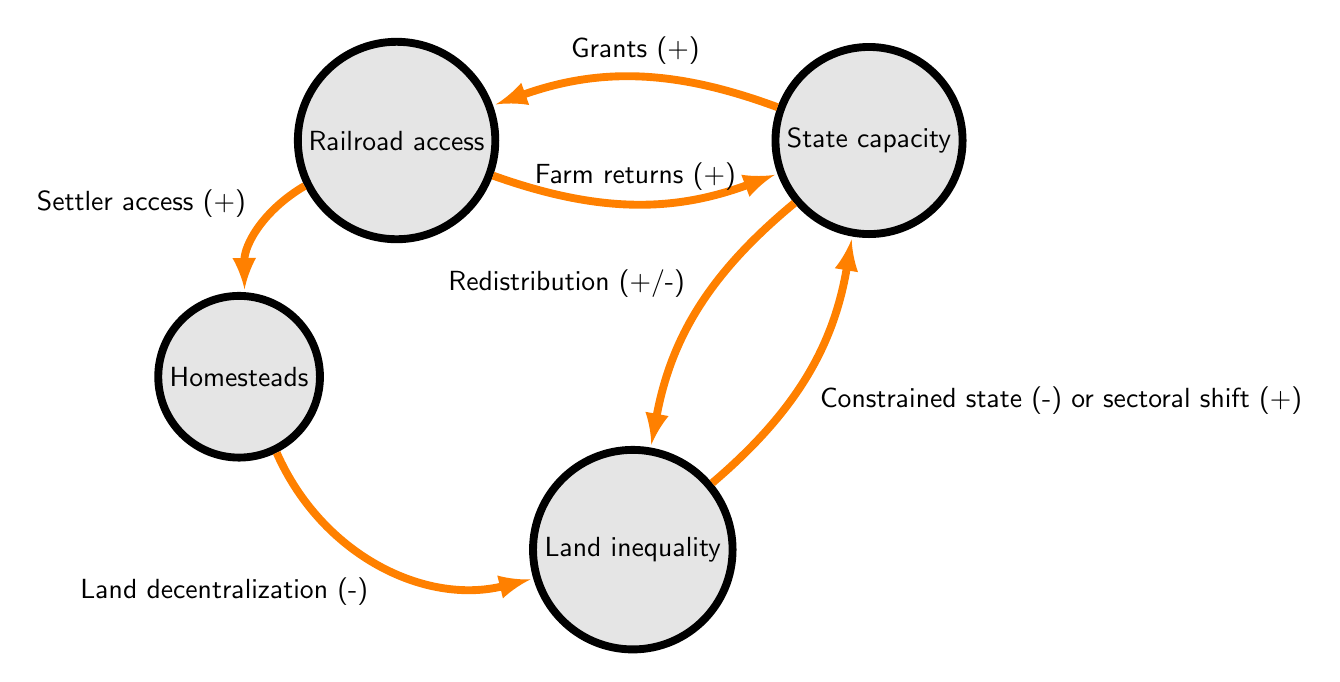
\begin{tikzpicture}[font=\sffamily]
		
		% Setup the style for the states
		\tikzset{node style/.style={state, 
				minimum width=2cm,
				line width=1mm,
				fill=gray!20!white}}
		
		% Draw the states
		\node[node style] at (0, 0)     (railroads)     {Railroad access};
		\node[node style] at (6, 0)     (capacity)     {State capacity};
		\node[node style] at (3, -5.196) (inequality) {Land inequality};
		\node[node style] at (-2, -3) (homesteads) {Homesteads};
		
		% Connect the states with arrows
		\draw[every loop,
		auto=right,
		line width=1mm,
		>=latex,
		draw=orange,
		fill=orange]
		(railroads)     edge[bend right=30]            node {Settler access (+) } (homesteads)
		(railroads)     edge[bend right=20, auto=left] node {Farm returns (+)} (capacity)
		(capacity)     edge[bend right=20]            node {Grants (+) } (railroads)
		(capacity)     edge[bend right=20, auto=center] node {Redistribution (+/-) } (inequality)
		(inequality) edge[bend right=20, auto=center]            node {Constrained state (-) or sectoral shift (+)} (capacity)
		(homesteads) edge[bend right=40, auto=right] node {Land decentralization (-)} (inequality);
	%	(homesteads) edge[bend right=20, auto=left] node {Demand (+)} (railroads);
		\end{tikzpicture}
\caption{Causal mechanisms underlying the relationship between homesteads and state capacity \label{fig:causal-graph}}
\end{figure}
 % Tables and Figures: introduction
\chapter{Supplementary Tables and Figures for Chapter \ref{land-reform}}


\begin{figure}[htbp]
	\centering
	\begin{subfigure}[t]{0.48\textwidth}
		\centering
		\includegraphics[width=\textwidth]{/media/jason/Dropbox/github/land-reform/paper/plots/basque_N_16_T_43_numruns_20_num_treated_8_simultaneuous_1.png}
		\caption{Basque Country terrorism data, $N_t = 8$} 
	\end{subfigure}
	~ 
	\begin{subfigure}[t]{0.48\textwidth}
		\centering
		\includegraphics[width=\textwidth]{/media/jason/Dropbox/github/land-reform/paper/plots/california_N_38_T_31_numruns_20_num_treated_19_simultaneuous_1.png}
		\caption{California smoking ban data, $N_t = 19$}
	\end{subfigure}
	~
	\begin{subfigure}[t]{0.48\textwidth}
		\centering
		\includegraphics[width=\textwidth]{/media/jason/Dropbox/github/land-reform/paper/plots/germany_N_16_T_44_numruns_20_num_treated_8_simultaneuous_1.png}
		\caption{West German reunification data, $N_t = 8$} 
	\end{subfigure}
	\caption{Placebo tests under simultaneous treatment adoption. \label{synth-sim}} 
\end{figure}

\begin{figure}[htbp]
	\begin{center}
		\includegraphics[width=\textwidth]{/media/jason/Dropbox/github/land-reform/paper/plots/homestead-heatmap.png}
	\end{center}
	\caption{Per-capita homestead entries in state $i$ and year $t$, 1869-1922. \label{fig:homestead-heatmap}}
\end{figure}

\begin{figure}[htbp]
	\centering
	\begin{subfigure}[t]{0.48\textwidth}
		\centering
		\includegraphics[width=\textwidth]{/media/jason/Dropbox/github/land-reform/paper/plots/exp_pc_N_17_T_159_numruns_20_num_treated_9_simultaneuous_1.png}
		\caption{Expenditures, simultaneous adoption}
	\end{subfigure}
	~ 
	\begin{subfigure}[t]{0.48\textwidth}
		\centering
		\includegraphics[width=\textwidth]{/media/jason/Dropbox/github/land-reform/paper/plots/rev_pc_N_18_T_158_numruns_20_num_treated_9_simultaneuous_1.png}
		\caption{Revenues, simultaneous adoption}
	\end{subfigure}
	~ 
	\begin{subfigure}[t]{0.48\textwidth}
		\centering
		\includegraphics[width=\textwidth]{/media/jason/Dropbox/github/land-reform/paper/plots/exp_pc_N_17_T_159_numruns_20_num_treated_9_simultaneuous_0.png}
		\caption{Expenditures, staggered adoption}
	\end{subfigure}
	~ 
	\begin{subfigure}[t]{0.48\textwidth}
		\centering
		\includegraphics[width=\textwidth]{/media/jason/Dropbox/github/land-reform/paper/plots/rev_pc_N_19_T_158_numruns_20_num_treated_10_simultaneuous_0.png}
		\caption{Revenues, staggered adoption}
	\end{subfigure}
	\caption{Placebo tests under simultaneous and staggered treatment adoption, with $N_t = 9$. \label{mc-sim}} 
\end{figure}

\begin{figure}[htbp]
	\centering
	\includegraphics[width=0.9\textwidth]{/media/jason/Dropbox/github/land-reform/paper/plots/mc-rev-pc.png}
	\caption{MC-NNM estimates of treatment exposure on state government revenue, 1809 to 1982:
		{\color{Darjeeling15}{\sampleline{}}}, observed treated;
		{\color{Darjeeling11}{\sampleline{dashed}}}, observed control;
		{\color{Darjeeling15}{\sampleline{dotted}}}, counterfactual treated;
		{\color{Darjeeling15}{\sampleline{dash pattern=on .7em off .2em on .05em off .2em}}}, $\hat{\bar{\alpha}}_{t}$.\label{mc-estimates-rev-pc}} 
\end{figure}

\begin{figure}[htbp]
	\begin{center}
		\includegraphics[width=1\textwidth]{/media/jason/Dropbox/github/land-reform/paper/plots/ineq-capacity.png} 
	\end{center}
	\caption{Land inequality (lagged by 10 years) vs. log per-capita revenue and expenditure, 1860-1950. Each point is a state-year observation. Lines represent generalized additive model (GAM) fits to the data and shaded regions represent corresponding 95\% confidence intervals.   \label{fig:ineq-capacity}}
\end{figure} 
 % Tables and Figures: land-reform
\chapter{Supporting Materials for Chapter \ref{ga-lottery}}

%1
\begin{table}[htbp] 
	\caption{Counties created by 1805 and 1807 lotteries. \label{counties-tab}}
	\begin{tabularx}{\linewidth}{l*{7}{Y}}
		\toprule
		\multicolumn{7}{l}{\textbf{Panel A: 1805}} \\
		\midrule
		Counties  & No. Districts & Lot sizes (acres)& Lot length (chains square)& Lot orientation (degrees) & Grant fee (\$) & Est. value of lot (\$)\\
		\hline
		Baldwin & 5  &  202.5  & 45& 45 / 60  & 8.10  & 839.17\\ 
		Wayne & 3 &  490  &70 &13 / 77  & 19.60 & 842.64 \\ 
		Wilkinson & 5  &  202.5  & 45&45 / 60 & 8.10 & 811.25 \\   
	\end{tabularx}
	\begin{tabularx}{\linewidth}{l*{7}{Y}}
		\toprule
		\multicolumn{7}{l}{\textbf{Panel B: 1807}} \\
		\midrule
		Counties  & No. Districts & Lot sizes (acres)& Lot length (chains square)& Lot orientation (degrees) & Grant fee (\$) & Est. value of lot (\$) \\
		\hline
		Baldwin & 15  &  202.5  & 45& 45 / 60  & 12.15  & 827.35\\ 
		Wilkinson & 23 &  202.5  & 45&45 / 60 & 12.15 & 799.82 \\    
		\bottomrule
	\end{tabularx} 
	\footnotesize{Notes: counties and land lots specified by Acts of 11 May 1803 and 9 June 1806. Lot orientation is degrees from the meridian. Lot values are estimated by averaging the cash value of farms minus the value of farming implements and machinery by the number of (improved and unimproved) acres of land in farms \citep{haines2004,bleakley2013up}. The 1850 values are deflated to 1805 dollars (Panel A) and 1807 dollars (Panel B) using a historical consumer price index \citep{officer2012}.}
\end{table}

%2
\begin{table}[htbp] 
	\begin{center}
		\caption{Distribution of census wealth by officeholding status.}   \label{officeholders-1820-1850}
		\resizebox{1\width}{!}{\input{/media/jason/Dropbox/ga-lottery-local/online-appendix/officeholders-1820-1850}}\\
	\end{center}
	\footnotesize{Notes: slave wealth adjusted to 1850\$ values \citep{williamson2016}. $p$-value is obtained from a Mann-Whitney-Wilcoxon test under the null hypothesis that officeholder and non-officeholder distributions are equal.} 
\end{table}

%9
\begin{table}[htbp]
	\begin{center}
		\caption{Record classification ensemble.\label{ensemble-tab-link}} 
		\begin{tabular}{llcc}
			\hline
			Algorithm & Parameters & MSE & Weight \\ 
			\hline
			\rowcolor{Gray}
			Super Learner & default & 0.02 & - \\
			Generalized boosted regression &  default & 0.02 & 0.05 \\ 
			GLM with elasticnet regularization	 &  $\alpha=0$ & 0.02 & 0 \\  % ridge
			GLM with elasticnet regularization	 &  $\alpha=0.25$ & 0.02& 0 \\ 
			GLM with elasticnet regularization 	&  $\alpha=0.5$ & 0.02 & 0 \\ 
			GLM with elasticnet regularization 	 &  $\alpha=0.75$ & 0.02 & 0 \\ 
			GLM with elasticnet regularization 	 &  $\alpha=1$ & 0.02 & 0.52 \\  % lasso
			Neural network  &  default & 0.13 & 0 \\ 
			Random forests 	& default & 0.02 & 0.32 \\ 
			Random forests 	 & $\# \, \text{variables sampled} =1$ & 0.04 & 0.09 \\ 
			Random forests 	  & $\# \, \text{variables sampled}=5$  & 0.02 & 0 \\ 
			Random forests 	 & $\# \, \text{variables sampled}=10$ & 0.03 & 0 \\ 
			\hline
		\end{tabular} 
	\end{center}
	\footnotesize{Notes: cross-validated risk and weights used for each algorithm in Super Learner prediction ensemble for record classification model. \textit{MSE} is the ten-fold cross-validated mean squared error for each algorithm. \textit{Weight} is the coefficient for the Super Learner, which is estimated using non-negative least squares based on the Lawson-Hanson algorithm. $\alpha$ is the elastic net mixing parameter, where $\alpha = 0$ is the ridge penalty and $\alpha = 1$ is the Lasso penalty. $\# \, \text{variables sampled}$ is the number of predictors sampled for splitting at each node.}
\end{table}

%12
\begin{table}[htbp] 
	\begin{center}
		\caption{Robustness: ITT treatment effects on officeholding.}   \label{officeholding-robust-table}
		\resizebox{0.8\width}{!}{\input{/media/jason/Dropbox/ga-lottery-local/online-appendix/officeholder-robust-table}}
	\end{center}
	\footnotesize{Notes: \textit{Officeholder (match prob.)} is the officeholder match probability. See notes to Table \ref{candidate-robust-table}.}  
\end{table} 

%13
\begin{table}[htbp] 
	\begin{center}
		\caption{Robustness: ITT treatment effects on candidacy.}   \label{candidate-robust-table}
		\resizebox{0.8\width}{!}{\input{/media/jason/Dropbox/ga-lottery-local/online-appendix/candidate-robust-table}}
	\end{center}
	\footnotesize{Notes: \textit{Candidate (match prob.)} is the candidate match probability. Covariates included are those that yield $p <0.10$ in Fig. \ref{balance-plot}.}  
\end{table}  

%14
\begin{table}[htbp] 
	\begin{center}
		\caption{Robustness: ITT treatment effects on slave wealth (1820\$).}   \label{slave-robust-table}
		\resizebox{0.8\width}{!}{\input{/media/jason/Dropbox/ga-lottery-local/online-appendix/slave-robust-table}}
	\end{center}
	\footnotesize{Notes: \textit{Slave wealth (weighted)} is the same measure weighted by the census match probability. See notes to Table \ref{candidate-robust-table}.}  
\end{table}   

\begin{figure}[htbp] %15
	\begin{center}
		\caption{Power analysis by simulation for binary response variable.\label{power-plot-bin}}		
		\includegraphics[width=1\textwidth]{/media/jason/Dropbox/ga-lottery-local/online-appendix/power-plot-bin.png} 
	\end{center}
	\footnotesize{Notes: $N=21,732$ and $\mathcal{I} =100$ iterations. The horizontal line indicates the 80\% power that is normally required to justify a study.}
\end{figure}

\begin{figure}[htbp] % 16
	\begin{center}
		\caption{Quantile regression treatment effect estimates on slave wealth for 1805 winners \& losers. \label{qreg-plot} }
		\includegraphics[width=1\linewidth]{/media/jason/Dropbox/ga-lottery-local/online-appendix/qreg-plot.png} \\
	\end{center}
	\footnotesize{Notes: estimates from a quantile regression of the treatment effect on imputed slave wealth for participants linked to the 1820 Census ($N=5,252$). The points are quantile-specific estimates of the treatment effect and the error bars represent 95\% confidence intervals constructed from bootstrapped standard errors. Quantiles above 0.98 are omitted for display purposes. The line is a LOESS-smoothed estimate of the treatment effect.}
\end{figure}
 % Tables and Figures: ga-lottery
\chapter{Power Analysis by Simulation}\label{oa-power}

The purpose of a power analysis by simulation is to estimate $\mathrm{P}(\mathrm{Reject \, H_0} | \mathrm{H_0 \, is \, false})$ at a fixed significance level ($\alpha =0.05$) and sample size ($N=21,732$) for different treatment effects $\Delta_{1, \ldots, j}$. In this case $N$ is the size of the observed sample of participants, excluding women and orphans. The simulation proceeds as follows:

\begin{enumerate}
	\item Take a random sample of size $N$ without replacement from from the observed distribution of treatment assignments, weighted by the observed propensity score, to create a vector of simulated treatment assignments.
	\item Simulate response values with $\Delta_{j}$ as the difference-in-means between the simulated treated and control units. Generate random values from the binomial distribution with the probability of success on each trial equal to the mean of the response in the observed sample.
	\item Run linear model on the simulated data and extract the $p$ value.
\end{enumerate}

Repeat the simulation $\mathcal{I}$ times and calculate power of the test by dividing the count of the number of $p$ values that are less than $\alpha$ over $\mathcal{I}$. Normally, 80\% power is required to justify a study.  Fig. \ref{power-plot-bin} provides the results of power analysis simulations for the officeholding response.  % Power analysis by simulation: ga-lottery
\chapter{Supplementary Tables and Figures for Chapter \ref{rnns-causal}}

\begin{figure}[htbp]
	\centering
	\includegraphics[width=0.9\textwidth]{/media/jason/Dropbox/github/rnns-causal/paper/plots/basque-sim.png}
	\caption{Placebo tests on Basque Country terrorism data: 
		{\protect\tikz \protect\draw[color={rgb:red,4;green,0;yellow,1}] (0,0) -- plot[mark=o, mark options={scale=2}] (0.25,0) -- (0.5,0);}, DID;
		{\protect\tikz \protect\draw[color={rgb:red,244;green,226;blue,66}] (0,0) -- plot[mark=triangle*, mark options={scale=2,fill=white}] (0.25,0) -- (0.5,0);}, ED; 
		{\protect\tikz \protect\draw[color={rgb:red,0;green,5;blue,1}] (0,0) -- plot[mark=+, mark options={scale=2}] (0.25,0) -- (0.5,0);}, MC-NNM;
		{\protect\tikz \protect\draw[color={rgb:red,66;green,200;blue,244}] (0,0) -- plot[mark=x, mark options={scale=2}] (0.25,0) -- (0.5,0);}, RVAE;
		{\protect\tikz \protect\draw[color={rgb:red,66;green,107;blue,244}] (0,0) -- plot[mark=diamond, mark options={scale=2}] (0.25,0) -- (0.5,0);}, SCM;
		{\protect\tikz \protect\draw[color={rgb:red,244;pink,66;blue,223}] (0,0) -- plot[mark=triangle, mark options={scale=2, rotate=180}] (0.25,0) -- (0.5,0);}, VT-EN.\label{basque-sim}}
\end{figure}

\begin{figure}[htbp]
	\centering
	\includegraphics[width=0.9\textwidth]{/media/jason/Dropbox/github/rnns-causal/paper/plots/germany-sim.png}
	\caption{Placebo tests on West German reunification data: 
		{\protect\tikz \protect\draw[color={rgb:red,4;green,0;yellow,1}] (0,0) -- plot[mark=o, mark options={scale=2}] (0.25,0) -- (0.5,0);}, DID;
		{\protect\tikz \protect\draw[color={rgb:red,244;green,226;blue,66}] (0,0) -- plot[mark=triangle*, mark options={scale=2,fill=white}] (0.25,0) -- (0.5,0);}, ED; 
		{\protect\tikz \protect\draw[color={rgb:red,0;green,5;blue,1}] (0,0) -- plot[mark=+, mark options={scale=2}] (0.25,0) -- (0.5,0);}, MC-NNM;
		{\protect\tikz \protect\draw[color={rgb:red,66;green,200;blue,244}] (0,0) -- plot[mark=x, mark options={scale=2}] (0.25,0) -- (0.5,0);}, RVAE;
		{\protect\tikz \protect\draw[color={rgb:red,66;green,107;blue,244}] (0,0) -- plot[mark=diamond, mark options={scale=2}] (0.25,0) -- (0.5,0);}, SCM;
		{\protect\tikz \protect\draw[color={rgb:red,244;pink,66;blue,223}] (0,0) -- plot[mark=triangle, mark options={scale=2, rotate=180}] (0.25,0) -- (0.5,0);}, VT-EN.\label{germany-sim}}
\end{figure}

\begin{figure*}[htbp]
	\centering
	\begin{subfigure}[t]{0.48\textwidth}
		\centering
		\includegraphics[width=\textwidth]{/media/jason/Dropbox/github/rnns-causal/paper/plots/educ-dens.png}
		\caption{Unweighted} 
	\end{subfigure}
	~ 
	\begin{subfigure}[t]{0.48\textwidth}
		\centering
		\includegraphics[width=\textwidth]{/media/jason/Dropbox/github/rnns-causal/paper/plots/educ-dens-w.png}
		\caption{Weighted by propensity score}
	\end{subfigure}
	\caption{Pre-period densities of log per-capita state government education spending by treatment status: {\protect\tikz \protect\draw[color=black] (0,0) -- plot[mark=square, mark options={scale=2, fill=white}] (0.25,0) -- (0.5,0);}, Control;
		{\protect\tikz \protect\draw[color={rgb:red,104;green,122;blue,255}] (0,0) -- plot[mark=square*, mark options={scale=2,fill={rgb:red,104;green,122;blue,255}}] (0.25,0) -- (0.5,0);}, Treated \label{educ-dense}} 
\end{figure*}

\begin{figure}[htbp]
	\centering
	\includegraphics[width=0.9\textwidth]{/media/jason/Dropbox/github/rnns-causal/paper/plots/educ-sim.png}
	\caption{Placebo tests on education spending data: 		{\protect\tikz \protect\draw[color={rgb:red,4;green,0;yellow,1}] (0,0) -- plot[mark=o, mark options={scale=2}] (0.25,0) -- (0.5,0);}, DID;
		{\protect\tikz \protect\draw[color={rgb:red,244;green,226;blue,66}] (0,0) -- plot[mark=triangle*, mark options={scale=2,fill=white}] (0.25,0) -- (0.5,0);}, ED; 
		{\protect\tikz \protect\draw[color={rgb:red,0;green,5;blue,1}] (0,0) -- plot[mark=+, mark options={scale=2}] (0.25,0) -- (0.5,0);}, MC-NNM;
		{\protect\tikz \protect\draw[color={rgb:red,66;green,200;blue,244}] (0,0) -- plot[mark=x, mark options={scale=2}] (0.25,0) -- (0.5,0);}, RVAE;
		{\protect\tikz \protect\draw[color={rgb:red,66;green,107;blue,244}] (0,0) -- plot[mark=diamond, mark options={scale=2}] (0.25,0) -- (0.5,0);}, SCM;
		{\protect\tikz \protect\draw[color={rgb:red,244;pink,66;blue,223}] (0,0) -- plot[mark=triangle, mark options={scale=2, rotate=180}] (0.25,0) -- (0.5,0);}, VT-EN.
		\label{educ-sim}}
\end{figure} % Tables and Figures: rnns-causal
\chapter{RNNs Implementation Details for Chapter \ref{rnns-causal}} \label{imp}

The networks are implemented with the \texttt{Keras} neural network library \citep{chollet2015keras} in Python on top of a TensorFlow backend. When implementing encoder-decoder networks, the encoder takes the form of a two-layer Long Short-Term Memory (LSTM) network \citep{schmidhuber1997long}, each with 128 hidden units, and the decoder is a single-layer Gated Recurrent Unit (GRU) \citep{chung2014} also with 128 hidden units. Each recurrent layer uses a linear activation function ($f_1$) with weights initialized using Xavier initialization \citep{glorot2010}. The loss function internally computes the predicted outputs as a linear function ($f_2$) of the log probabilities. 

RNN weights are learned with mini-batch gradient descent on the WMSE using \texttt{Adam} stochastic optimization with the learning rate set to $5\,\cdot\,10^{-4}$ \citep{kingma2014adam}. As a regularization strategy, I apply dropout to the inputs and L2 regularization losses to the network weights. The networks are trained for 1,000 epochs, which takes 10 minutes to run on a laptop CPU. The model is validated on the last 20\% of the training set input-out pairs.  

The RVAE is implemented similarly, but with the following differences: the encoder takes the form of a single-layer LSTM with 32 hidden units and the decoder is a two-layer LSTM with the number of hidden units equal to 32 and the number of predictors, respectively. The latent space $\boldsymbol{z}$ is implemented as a densely-connected layer with a dimension of 200 units and $f_3(\cdot)$ takes the form of a log-normal distribution. The RVAE is trained with stochastic gradient descent for 5,000 epochs, which takes seven minutes to run on the same CPU. % RNNs implementation details: rnns-causal
\chapter{Hypothesis Testing for Chapter \ref{rnns-causal}} \label{eval}

\citet{abadie2010synthetic} propose a randomization inference approach for calculating the exact distribution of placebo effects under the sharp null hypothesis of no effect. \citet{cavallo2013catastrophic} extends the placebo-based testing approach to the case of multiple (placebo) treated units by constructing a distribution of \emph{average} placebo effects under the null hypothesis. \citet{firpo2018synthetic} derive the conditions under which the randomization inference approach is valid from a finite sample perspective and \citet{hahn2017synthetic} analyze the approach from a repeated sampling perspective.

Randomization $p$-values are obtained following these steps:

\begin{enumerate} 
	\item Estimate the observed test static $\boldsymbol{\hat{\upphi}}$ from (\ref{eq:pointwise}). Averaging over the time dimension results in a $\text{T}_\star$-length array of observed average treatment effects. 
	\item Calculate every possible average placebo treated effect $\upmu$ by randomly sampling without replacement which $\text{J}-1$ control units are assumed to be treated. There are $\mathcal{Q} = \sum\limits_{\text{g}=1}^{\text{J}-1} {\text{J} \choose \text{g}}$ possible average placebo effects.\footnote{Since calculating $\mathcal{Q}$ can be computationally burdensome for relatively high values of $J$, I artificially set $\mathcal{Q} = 10,000$ in cases when $\text{J} > 16$.} The result is a matrix of dimension $\mathcal{Q} \times \text{T}_\star$
	\item Sum over the time dimension the number of $\upmu$ that are greater than or equal to $\boldsymbol{\hat{\upphi}}$.  \label{counts}
\end{enumerate}

Each element of the vector obtained from Step \ref{counts} is divided by $\mathcal{Q}$ to estimate a $\text{T}_\star$-length vector of exact two-sided $p$ values, $\hat{p}$. 

\subsection{Randomization confidence intervals}

Under the assumption that treatment has a constant additive effect $\Delta$, I construct an interval estimate for $\Delta$ by inverting the randomization test. Let $\updelta_\Delta$ be the test statistic calculated by subtracting all possible $\upmu$ by $\Delta$. I derive a two-sided randomization confidence interval by collecting all values of $\updelta_\Delta$ that yield $\hat{p}$ values greater than or equal to significance level $\upalpha=0.05$. I find the endpoints of the confidence interval by randomly sampling 500 values of $\Delta$. % Hypothesis testing: rnns-causal

\end{document}
